% Chapter Template

\chapter{Private information in Petri nets. Subnets} % Main chapter title

\label{Chapter: Subnets} % Change X to a consecutive number; for referencing this chapter elsewhere, use \ref{ChapterX}

\lhead{Chapter 3. \emph{Private information in Petri nets. Subnets}} % Change X to a consecutive number; this is for the header on each page - perhaps a shortened title

%----------------------------------------------------------------------------------------
%       SECTION 1
%----------------------------------------------------------------------------------------

\section{Introduction}
By default, a Petri net is described in a comprehensive and public way.
In this chapter I am going to describe a way to declare private information of a Petri net.
This information is candidate to be hidden, complying in this way with the
goal of privacy.
Furthermore, this theory can be applied afterwards in  order to sign parts of a Petri net (subnets) achieving the objectives of integrity, authentication
and non repudiation.   

First of all I have to create a like framework of definitions, properties
and methodologies in order to achieve this goal. The main idea is the concept
of subnet an its interaction front-end.

Once defined this subnets, the Petri net can be divided into public and private
chunks only by ordering the places and transitions in one subnet or another. \section{Petri subnets}

\subsection{Definitions and properties}

Let $ P $ and $ T $ the non-empty finite sets of places and
transitions of a Petri net, respectively. Let $ | P | = n $ (the number of places
of the net) and $ | T | = m $ (number of transitions of the net). Let $ \alpha $ and $ \beta $ pre and post incidence matrices respectively. Let $ N = \langle P, T, \alpha, \beta \rangle $ be a
Petri net and let $ C $ the incidence matrix of $ N $

\begin{definition}[Subnet \cite{G-Silva1985}]
A subnet of $N=\langle P,T,\alpha,\beta\rangle$
is a net $\overline{N}=\langle\overline{P},\overline{T},\overline{\alpha},\overline{\beta}\rangle$
so that $\overline{P}\subseteq P$ y $\overline{T}\subseteq T$, $\overline{\alpha}$
y $\overline{\beta}$ are restrictions of $\alpha$ and $\beta$ over
$\overline{P}\times\overline{T}$.
\end{definition}
In other words, a subnet is a subset of places and transitions
together with the arches that connect them together.

Let's look at the implications of the latter definition
since it is one of the most important with regard to this work.

A subnet corresponds \cite{HID-Inigo2011MT}, in terms of matrices, with the resulting submatrix keeping only the rows and columns corresponding to places and transitions of the selected subnet.
\begin{example} Let's take the Petri net which has the following incidence matrix:
\[
C=
\kbordermatrix{
   &t_1&t_2&t_3&t_4&t_5&t_6\\
p_1&-1 & 0 & 1 & 0 & 0 & 0\\
p_2&-1 & 0 & 0 & 1 & 0 & 0\\
p_3&1 & 0 & 0 & 0 & 0 & 0\\
p_4&0 & -1 & -1 & 0 & 0 & 0\\
p_5&0 & 1 & 0 & -1 & -1 & 1\\
p_6&0 & 0 & 0 & 0 & 1 & -1\\
}
\]

If we select the places $ p_1 $, $ p_3 $, $ p_4$ and $ p_5$
and transitions $ t_1 $, $ t_2 $, and $ t_6 $ we have the
subnet defined by this incidence matrix
\[
C'=
\kbordermatrix{
   &t_1&t_2&t_6\\
p_1&-1 & 0 & 0 \\
p_3&1 & 0 & 0 \\
p_4&0 & -1 & 0 \\
p_5&0 & 1 & 1 \\
}
\]

by simply erasing $p_2$ and $p_6$ rows and $t_3$, $t_4$ and $t_5$ columns.
\end{example}

In \cite{HID-Inigo2011MT} is shown that the set of all
possible permutations of rows and/or columns of a matrix of incidence
corresponding to a Petri net, either the pre or post incidence matrix, make an equivalence relation. In other words, given an incidence matrix, both rows and columns can be rearranged
 and this rearrangement describes exactly the original Petri net.

In this way, we can study the incidence matrices reordering
rows and columns as preferred one at any time, without loss
of generality.

\begin{figure*}[htbp]
\centering
\[
\kbordermatrix{
   & t_1&t_2&t_3&t_4&t_5&t_6\\
p_1&-1 & 0 & 1 & 0 & 0 & 0\\
p_2&-1 & 0 & 0 & 1 & 0 & 0\\
p_3&1 & 0 & 0 & 0 & 0 & 0\\
p_4&1 & -1 & 0 & 0 & 0 & 0\\
p_5&0 & 1 & 0 & 0 & 0 & 0\\
p_6&0 & 0 & -1 & 0 & 0 & 0\\
p_7&0 & 0 & 0 & -1 & -1 & 1\\
p_8&0 & 0 & 0 & 0 & 1 & -1\\
}
\equiv
\kbordermatrix{
   &t_1&t_6&t_3&t_5&t_4&t_2\\
p_8& 0 &-1 & 0 & 1 & 0 & 0\\
p_1&-1 & 0 & 1 & 0 & 0 & 0\\
p_3& 1 & 0 & 0 & 0 & 0 & 0\\
p_6& 0 & 0 & -1& 0 & 0 & 0\\
p_4& 1 & 0 & 0 & 0 & 0 & -1\\
p_5& 0 & 0 & 0 & 0 & 0 & 1\\
p_2&-1 & 0 & 0 & 0 & 1 & 0\\
p_7& 0 & 1 & 0 & -1& -1& 0\\
}
\]
\rule{35em}{0.5pt}
\caption{Two equivalent incidence matrices to describe the same Petri net}
\label{fig:matriz_incidencia_relacion_equivalencia}
\end{figure*}

From all these definitions and proofs we can draw several
trivial conclusions: 
\begin{enumerate}
\item A subnet, like generic Petri net does not have to be square.
\item If a row or column of the incidence matrix of the subnet is all zeros, it doesn't
mean that that place or that transition is isolated. This occurs only with pure nets.
If there is an arc from one transition to a place and an arc from that place
to the same transition with the same weight, the sum (the matrix
element associated to that place/transition) is zero , but there are
two arcs.
\item It does not matter the number of places and/or transitions that are chosen
for the subnet, as long as they are not empty sets. 
\end{enumerate}





\subsection{Splitting a net into subnets}

Let $N=\langle P,T,\alpha\beta\rangle$ a Petri net where $|P|=n$
and $|T|=m$. So $P=\{p_{1},p_{2}...p_{n}\}$ and $T=\{t_{1},t_{2}...t_{m}\}$.
Select two subsets $P'\subseteq P$ and $T'\subseteq T$
so that $|P'|=r\le n$ and $|T'|=s\le m$. With these premises
divide into two subnets the original one.

We have seen that we can identify a subnet by simply removing
rows and/or columns (places/transitions) of an incidence matrix.
Taking advantage of the equivalence relation defined in \cite{HID-Inigo2011MT},
we reorder the incidence matrix so that places and transitions of the subnet
are in the top-left.
Without loss of
generality, and for convenience, places and transitions can be renamed so that the incidence matrix
is as follows: 
\[
C=
\kbordermatrix{
& t_{1} & \cdots & t_{s} &  & t_{s+1} &  \cdots &  t_{m}\\
p_1 & a_{11} & \cdots & a_{1s} &\omit\vline & a_{1(s+1)} & \cdots & a_{1m}\\
\vdots & \vdots & \ddots & \vdots & \omit\vline & \vdots & \ddots & \vdots\\
p_r & a_{r1} & \cdots & a_{rs} & \omit\vline& a_{r(s+1)} & \cdots & a_{rm}\\
\cline{2-8}
p_{r+1} &a_{(r+1)1} & \cdots & a_{(r+1)s} & \omit\vline& a_{(r+1)(s+1)} & \cdots & a_{(r+1)m}\\
\vdots & \vdots & \ddots & \vdots & \omit\vline& \vdots & \ddots & \vdots\\
p_n & a_{n1} & \cdots & a_{ns} & \omit\vline& a_{n(s+1)} & \cdots & a_{nr}
}
\]


We now have the net divided into two disjoint and complementary subnets. They are disjoint because there is no place and no
common transition, and complementary because the union of the two we
gives the complete net. At this point note that the incidence matrix
is divided into four blocks
$
C=\left(\begin{array}{cc}
N_{1} & PIM_{12}\\
TIM_{12} & N_{2}
\end{array}\right)
$. The interpretation is as follows: 
\begin{itemize}
\item $N_1$ subnet made up of places $p_{1} .. p_{r}$ and
transitions $ t_{1} .. t_{s} $
\item $N_2$ subnet that is complementary to $N_1$, made up of the places $p_{r +1} .. p_{n} $ and transitions $t_{s+1} .. t_{m}$
\item $PIM_{12}$ (Places Influence Matrix) is the matrix that defines the interaction of the $N_1$ places with $N_2$ transitions. Basically it is the matrix
whose elements are those that are in the same rows of $N_1$ but outside
of it (rows $1..s$ and columns $s+1..m$).
\item $TIM_{12}$ (Transitions Influence Matrix) is the matrix that defines the interaction of $N_1$ transitions with $N_2$ places. It is the matrix whose elements are in the same columns of $N_1$ elements but outside of it (rows $r+1..n$ and columns $1..s$). 
\end{itemize}

We can notice that $PIM_{12}=TIM_{21}$ and $PIM_{21}=TIM_{12}$ by applying
the definition.


This can be generalized to multiple disjoint and complementary subnets without further to re-apply the same process to any of the subnets already defined. Thus, generically we can divide a network into $ i $ subnetworks, so we'll have a matrix of this style:
\[
\left(\begin{array}{ccc|ccc|c|ccc}
a_{11} & \cdots & a_{1s} & a_{1(s+1)} & \cdots & a_{1t} &  & a_{1u} & \cdots & a_{1m}\\
\vdots & \mathbf{N_1} & \vdots & \vdots & \ddots & \vdots & \cdots & \vdots & \ddots & \vdots\\
a_{p1} & \cdots & a_{ps} & a_{p(s+1)} & \cdots & a_{pt} &  & a_{pu} & \cdots & a_{pm}\\
\cline{1-10}a_{(p+1)1} & \cdots & a_{(p+1)s} & a_{(p+1)(s+1)} & \cdots & a_{(p+1)t} &  & a_{(p+1)u} & \cdots & a_{(p+1)m}\\
\vdots & \ddots & \vdots & \vdots & \mathbf{N_2} & \vdots & \dots & \vdots & \ddots & \vdots\\
a_{q1} & \cdots & a_{qs} & a_{q(s+1)} & \cdots & a_{qt} &  & a_{qu} & \cdots & a_{qm}\\
\cline{1-10} & \vdots &  &  & \vdots &  & \ddots &  & \vdots\\
\cline{1-10}a_{r1} & \cdots & a_{rs} & a_{r(s+1)} & \cdots & a_{rt} &  & a_{ru} & \cdots & a_{rm}\\
\vdots & \ddots & \vdots & \vdots & \ddots & \vdots & \cdots & \vdots & \mathbf{N_i} & \vdots\\
a_{n1} & \cdots & a_{ns} & a_{n(s+1)} & \cdots & a_{nt} &  & a_{nu} & \cdots & a_{nm}
\end{array}\right)
\]

In this situation, if we select two subnets $ N_ {j} $ and $ N_ {k} $,
we locate the zones of influence of each with respect to the other:
\[
\left(
\begin{array}{c|c|c|c|c}
\ddots & \cdots & \cdots & \cdots & \cdots \\
\hline
\vdots & SN_j & \cdots & PIM_{jk}=TIM_{jk} & \cdots \\
\hline
\vdots & \cdots & \ddots & \cdots & \cdots \\
\hline
\vdots & TIM_{jk}=PIM_{kj} & \cdots & SN_k & \cdots \\
\hline
\vdots & \vdots & \cdots & \vdots & \ddots \\
\end{array}
\right)
\]


Thus, the submatrix $ PIM_{jk} $ represents the arcs that connect places of the submatrix $ N_ {j} $ with $ N_k$ transitions and the matrix $ TIM_{kj} $ represents the arcs that connect places of $ SN_ {k} $ to $ SN_j$ transitions.

\notation{For simplicity, we will call
\begin{itemize}
 \item $PIM_i$ to all the elements in the same rows of $N_i$ but outside of it.
 \item $TIM_i$ to all the elements in the same columns of $N_i$ but outside of it.
\end{itemize}

We can notice again that $PIM_{jk}=TIM_{kj}$ and $PIM_{kj}=TIM_{jk}$ by applying
the definition.

\begin{definition}[Partition of a Petri net into subnets]
We say that a set $ P = \{N_1 N_2 ... N_k \} $ is a partition into subnets of $ N $ if the following holds:
\begin{itemize}
  \item $N_1 \cup N_2 \cup ... \cup N_k = N$
  \item $\forall i, j | 1\leqslant i, j \leqslant k \Rightarrow\ N_i \cap N_j = \emptyset$ (pairwise disjoint)
\end{itemize}

\end{definition}









\subsection{Subnet classification}

Depending on how each of the four pieces of matrix ($N_1$, $N_2$, $PIM$ and $TIM$) are, we can see some special cases.

\subsubsection{Disjointed subnets}


\begin{definition}[Disjointed subnet]
Pure subnet said disjointed if there is no arc between its own places and transitions
\end{definition}

Suppose that in the incidence matrix divided into the four pieces explained, are $N_1$ or $N_2$ be a null matrix. In this case the interpretation is that there arcs between places and transitions of the subnet, which would simply places and/or no transitions related to each other but with the additional subnetwork. Subnet talk then disjointed.

\begin{proposition}
A subnet is disjoint iif its incidence submatrix is the null matrix.
\end{proposition}
The demonstration is trivial.

\begin{example}
Consider the next well-printed Petri net and its incidence matrix:
\[
\begin{matrix}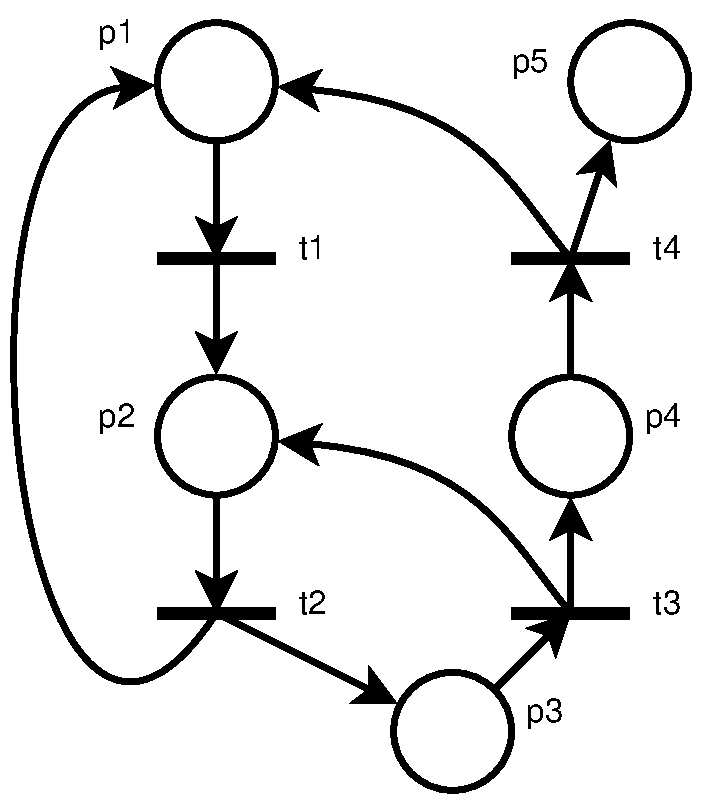
\includegraphics[width=0.3\textwidth]{Figures/EleccionSubredZonasInfluencia_1.eps}\end{matrix}
\ \ \ \ \ \ 
C=
\kbordermatrix{
   & t_1 & t_2 & t_3 & t_4\\
p_1& -1 &  1  &  0  &  1 \\
p_2&  1 & -1  &  1  &  0 \\
p_3&  0 &  1  & -1  &  0 \\
p_4&  0 &  0  &  1  & -1 \\
p_5&  0 &  0  &  0  &  1 \\
}
\]
We assume that we select as subnet the one formed by 4th and 5th places and transitions 1 and 2. Then the graph and the incidence matrix are thus:

\[
\begin{matrix}\includegraphics[width=0.50\textwidth]{Figures/subredInconexa.eps}\end{matrix}
\ \ \ \ \ \ 
C=
\kbordermatrix{
   & t_1 & t_2 & \vline & t_3 & t_4\\
p_4&  0 &  0  &  \vline & 1  & -1 \\
p_5&  0 &  0  &  \vline & 0  &  1 \\
\hline
p_1& -1 &  1  &  \vline & 0  &  1 \\
p_2&  1 & -1  &  \vline & 1  &  0 \\
p_3&  0 &  1  &  \vline & -1  &  0 \\
}
\]

Here we can see that although really $p_4 $, $ p_5 $, $ t_1 $ and $ t_2 $ are not isolated, there is no arc that connects them together. In the incidence matrix, the corresponding submatrix is the zero matrix. Therefore, whether or not there are elements isolated in the net, total subnet formed by $ p_4 $, $ p_5 $, $ t_1 $ and $t_2$ is a disjointed subnet.

\end{example}

We can extend this definition to a subnet that is part of a bigger net. It
doesn't matter in how many subnets it is separated: if one subnet is the null
matrix, this subnet is disjointed. This characteristic is implicit to the selected subnet and it doesn't depend on the rest of the net.

\subsubsection{Macroplace}

Once subnet concept is introduced, we can classify them by some properties.
In this case, a subnet which behaviour is like a place, relating only to
transitions can be defined as macroplace.
\begin{definition}[Macroplace]
A macroplace is a subnet that meets the following:
\begin{enumerate}
 \item arcs entering any node of the subnet from an external node come from a transition.
 \item arcs leaving any node on the subnet to an external node go to a transition.
\end{enumerate}
\end{definition}

\begin{proposition}
A subnet $N_1$ is a macroplace iif its transitions influence matrix (TIM) is the null matrix. In the same way, $N_2$ is a macroplace iif its places
influence matrix (PIM) is the null matrix
\[
N_1\mbox{ is macroplace} \iff \forall a_{ij} \in TIM_1, a_{ij} =
0
\]
\[
N_2\mbox{ is macroplace} \iff \forall a_{ij} \in PIM_1, a_{ij} =
0
\]
\end{proposition}
The demonstration is trivial.


Suppose that the incidence matrix divided into the four pieces explained, $TIM$ appears to be the zero matrix. Then we conclude that the subnet $N_1$ is only related by arcs with places of subnet $N_2$. All arcs entering $N_1$ come from transitions of $N_2$ and all arcs coming out from $N_1$ go to transitions of $N_2$. Stated another way, the subnet $N_1$ behaves like a place, but may contain places and transitions.

Note that this is not really a place, and that the subnet has not marked as such. The marking is on the places within the subnet and depends on the arches of arrival.
\begin{example}[Macroplace]
If we take the figure \ref{fig:macroplace} we can see that the subnet inside
the rectangle $N_1$ is related to the rest of the net only through transitions,
it is to say, there is no arc from an external place or from an internal
transition. Furthermore, $TIM_1$ is the null matrix. So this subnet is a
macroplace.
 
\begin{figure}
\[
\begin{matrix}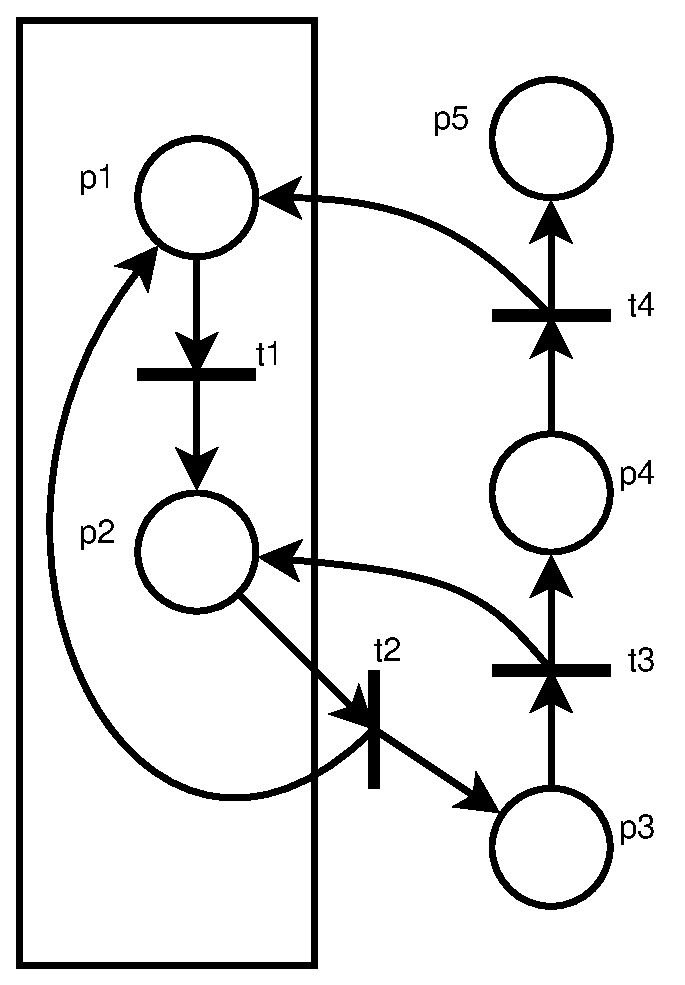
\includegraphics[width=0.3\textwidth]{Figures/macrolugar.eps}\end{matrix}
\ \ \ \ \ \ 
C=
\kbordermatrix{
   & t_1 & \vline & t_2 & t_3 & t_4\\
p_1& -1 & \vline &  1  &  0  &  1 \\
p_2&  1 & \vline & -1  &  1  &  0 \\
\hline
p_3&  0 & \vline &  1  & -1  &  0 \\
p_4&  0 & \vline &  0  &  1  & -1 \\
p_5&  0 & \vline &  0  &  0  &  1 \\
}
\]
\rule{35em}{0.5pt}
\caption{Macroplace}
\label{fig:macroplace}
\end{figure}

\end{example}

We can extend this definition to a subnet that is part of a bigger net too. However, in this time, it does matter the way in which the bigger net is separated. This characteristic is not implicit to the selected subnet and depends on the rest of the net.

//TODO Estos tres siguiente TODO no son estrictamente necesarios. Hacerlo solo si da
tiempo

//TODO explicar macroplace dependiendo del resto de subredes. Una subred puede comportarse como macrolugar sobre otra subred, pero no sobre una tercera.

//TODO macroplace absoluta si da igual el resto de subredes

//TODO Caracterizacion de macroplace absoluta

\subsubsection{Macrotransition}
In the same way as macroplaces, a subnet which behaviour is like a transition, relating only to
places can be defined as macrotransition.
\begin{definition}[Macrotransition]
A macrotransition is a subnet that meets with the following:
\begin{enumerate}
 \item arcs entering any node of the subnet from an external node come from a place.
 \item arcs leaving any node on the subnet to an external node go to a place.
\end{enumerate}
\end{definition}

\begin{proposition}
A subnet $N_1$ is a macrotransition iif its places influence matrix (PIM) is the null matrix. In the same way, $N_2$ is a macrotransition iif its transitions
influence matrix (TIM) is the null matrix
\[
N_1\mbox{ is macrotransition} \iff \forall a_{ij} \in PIM_1, a_{ij} =
0
\]
\[
N_2\mbox{ is macrotransition} \iff \forall a_{ij} \in TIM_1, a_{ij} =
0
\]
\end{proposition}
The demonstration is trivial

This is other option that can happen is that in the incidence matrix: $PIM$ appears to be the zero matrix. Then we conclude that the subnet $N_1$ is only related by arcs with places of subnet $N_2$. All arcs entering $N_1$ come from places of $N_2$ and all arcs coming out from $N_1$ go to places of $N_2$. Stated another way, the subnet $N_1$ behaves like a transition, but may contain places and transitions.

Like macroplaces, macrotransitions are not transitions as such. It is not necessary that all entries are marked to fire the macrotransition, and not all output places are marked after entering it. Everything depends on the inner workings of the macrotransition.

\begin{example}[Macrotransition]
If we take the figure \ref{fig:macrotransition} we can see that the subnet
inside the rectangle $N_2$ is related to the rest of the net only through places,
it is to say, there is no arc from an external transition or from an internal
place. Furthermore, $TIM_1$ is the null matrix. So this subnet is a
macrotransition.

\begin{figure}[htbp]
\centering
\[
\begin{matrix}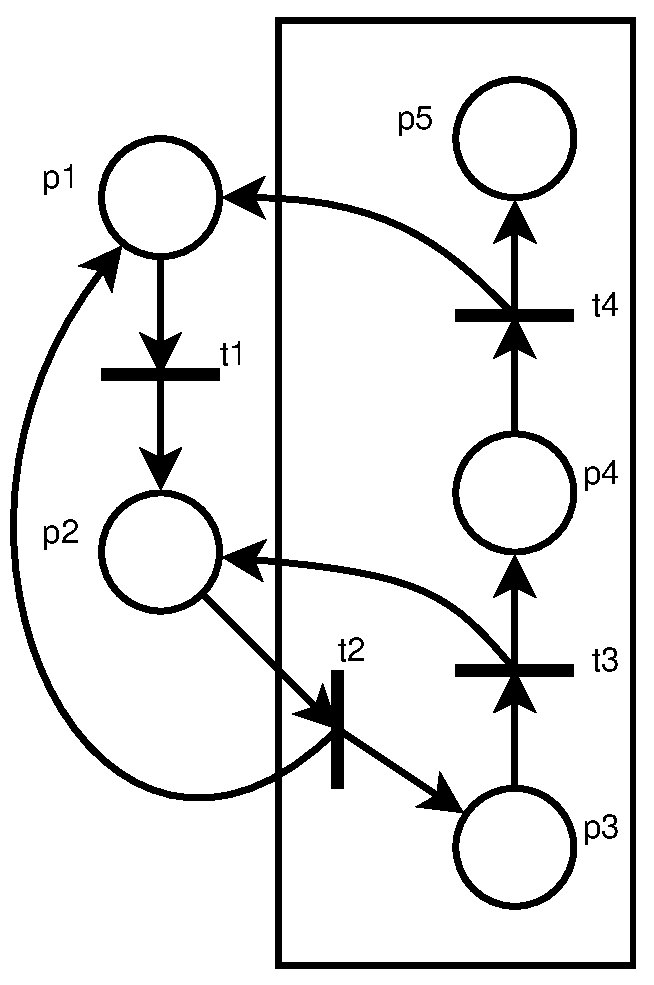
\includegraphics[width=0.3\textwidth]{Figures/macrotransicion.eps}\end{matrix}
\ \ \ \ \ \ 
C=
\kbordermatrix{
   & t_1 & \vline & t_2 & t_3 & t_4\\
p_1& -1 & \vline &  1  &  0  &  1 \\
p_2&  1 & \vline & -1  &  1  &  0 \\
\hline
p_3&  0 & \vline &  1  & -1  &  0 \\
p_4&  0 & \vline &  0  &  1  & -1 \\
p_5&  0 & \vline &  0  &  0  &  1 \\
}
\]
\rule{35em}{0.5pt}
\caption{Macrotransition}
\label{fig:macrotransition}
\end{figure}
\end{example}

We can extend this definition again to a subnet that is part of a bigger net too. Like with macroplaces, it does matter the way in which the bigger net is separated. 

//Estos cuatro siguientes TODO no son estrictamente necesarios. S�lo si da tiempo

//TODO explicar macrotransition dependiendo del resto de subredes. Una subred puede comportarse como macrotransition sobre otra subred, pero no sobre una tercera.

//TODO macrotransition absoluta si da igual el resto de subredes

//TODO Caracterizacion de macrotransicion absoluta

//TODO Explicar relacion entre una macrotransicion y un macrolugar en la
misma red, con subredes interrelacionadas por esta caracteristica. Una subred
es macrolugar sobre otra si y solo si esta ultima es macroplace sobre la
primera. Comprobarlo y demostrarlo en su caso


\subsubsection{Sinkhole subnet}

Another thing that can happen is that arrive only arcs to the selected subnet. Then we find that you can not leave the subnet. We speak then of a sinkhole
subnet.

\begin{definition}[Sinkhole subnet]
It is said that a subnet is a sinkhole subnet if no arc has its origin in an internal node (place or transition) of the subnet.
\end{definition}

It is easy to see that a subnet is sinkhole if and only if all elements of $PIM$ are greater or equal to zero and all elements of $TIM$ are less than or equal to zero.
\[
N_1\mbox{ is sinkhole } \iff \forall a_{ij} \in PIM_{1}, a_{ij} \geq
0 \land \forall a_{pq} \in TIM_{1}, a_{pq} \leq 0
\]

The demonstration is trivial
\begin{example}[Sinkhole Subnet]
If we have a look to the figure \ref{fig:sinkhole_subnet}, we can see that
there is no arc leaving the subnet $N_1$ defined by the rectangle. Furthermore,
$\forall a_{ij} \in PIM_{1}, a_{ij} \geq 0 \land \forall a_{pq} \in TIM_{1},
a_{pq} \leq 0$, so we have a sinkhole subnet.
\end{example}

If we can extend this definition to a subnet that is part of a bigger net,
in this case, it does matter the way in which the bigger net is separated. This characteristic is not implicit to the selected subnet and depends on the other subnets.

//TODO reescribir este parrafo anterior para que no sea
igual que los anteriores

//TODO estos tres siguiente TODO no son estrictamente necesarios. Hacerlo solo
si da tiempo

//TODO explicar sinkhole dependiendo del resto de subredes. Una subred puede comportarse como sinkhole sobre otra subred, pero no sobre una tercera.

//TODO Sinkhole absoluta si da igual el resto de subredes

//TODO Caracterizacion de Sinkhole subnet absoluta

\begin{figure}
\centering
\[
 \begin{matrix}
    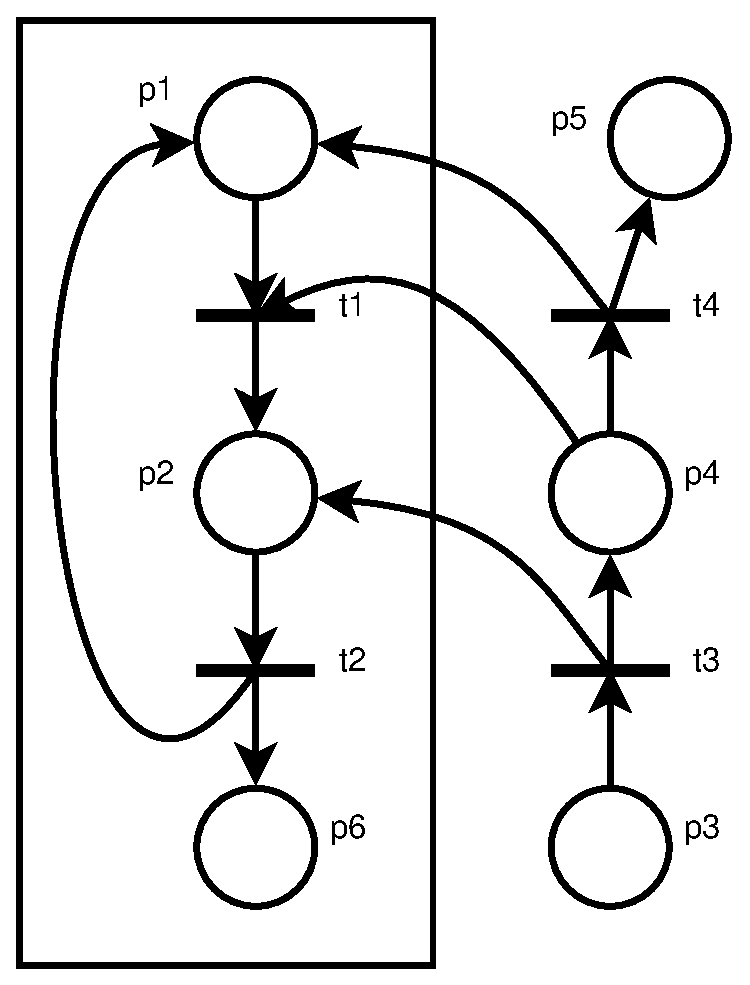
\includegraphics[width=0.3\textwidth]{Figures/subredSumidero.eps}
 \end{matrix}
  \ \ \ \ \ 
C=
\kbordermatrix{
   & t_1 & t_2 & \vline & t_3 & t_4\\
p_1&  -1 &  1  &  \vline & 0  & 1 \\
p_2&  1 &  -1  &  \vline & 1  &  0 \\
p_6&  0 &  1  &  \vline & 0  &  0 \\
\hline
p_3& 0 &  0  &  \vline & -1  &  0 \\
p_4&  -1 & 0  &  \vline & 1  &  -1 \\
p_5&  0 &  0  &  \vline & 0 &  1 \\
}
\]
\rule{35em}{0.5pt}
\caption{Sinkhole subnet}
\label{fig:sinkhole_subnet} 
\end{figure}


\subsubsection{Source subnet}
If instead of this what happens is no arc gets into the subnet, we have a source subnet. In a source subnet we can not enter.

\begin{definition}[Source subnet]
It is said that a subnet is a source subnet if no arc has its destination in an internal node (place or transition) of the subnet.
\end{definition}

\begin{figure}[htbp]
\centering
\[
 \begin{matrix}
    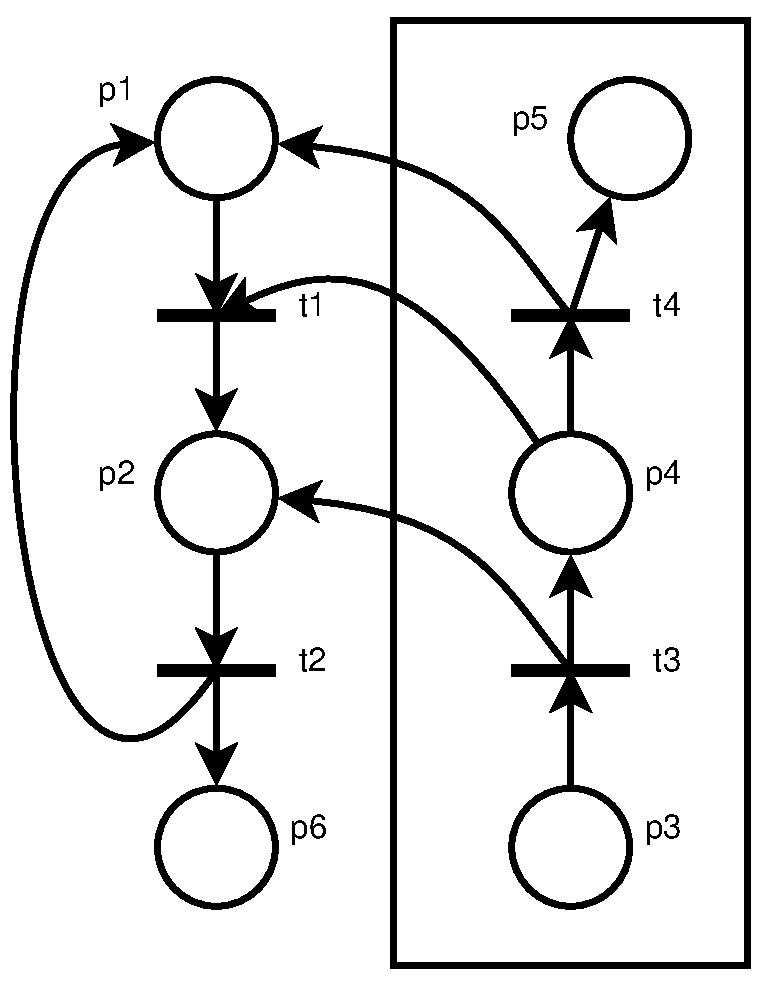
\includegraphics[width=0.3\textwidth]{Figures/subredFuente.eps}
 \end{matrix}
  \ \ \ \ \ 
C=
\kbordermatrix{
   & t_3 & t_4 & \vline & t_1 & t_2\\
p_3& -1 &  0  &  \vline & 0  &  0 \\
p_4&  1 & -1  &  \vline & -1  &  0 \\
p_5&  0 &  1  &  \vline & 0 &  0 \\
\hline
p_1&  0 &  1  &  \vline & -1  & 1 \\
p_2&  1 &  0  &  \vline & 1  &  -1 \\
p_6&  0 &  0  &  \vline & 0  &  1 \\
}
\]
\rule{35em}{0.5pt}
\caption{Source subnet}
\label{fig:source_subnet} 
\end{figure}


It is easy to see that a subnet is source if and only if all elements of $TIM$ are greater than or equal to zero and all elements of $PIM$ are less than or equal to zero.
\[
\mbox{$N_1$ is source } \iff \forall a_{ij} \in TIM_1, a_{ij} \geq 0  \land \forall a_{pq} \in PIM_1, a_{pq} \leq 0
\]

The demonstration is trivial

\begin{example}[Source Subnet]
In the same way that with the sinkhole subnet explained before, if we take
the figure \ref{fig:source_subnet} we can see that the subnet $N_1$ inside
the rectangle has no arc leaving it and $\forall a_{ij} \in TIM_1, a_{ij} \geq 0  \land \forall a_{pq} \in PIM_1, a_{pq} \leq 0$ so we have a source
subnet.
\end{example}








\subsection{Matrix parts description once defined the subnets}

As places and transitions can be reordered smoothly, we study a network N divided into 2 subnets, for simplicity and without loss of generality.
At this moment I am going  to study several topic in order to approach privacy,
by hiding a subnet. For consistency with \cite{HID-Inigo2011MT} we will follow this notation:
\[
\left(
\begin{array}{c|c}
 H & HP\\
 \cline{1-2} 
 HT & V
\end{array}
\right)
\]
where
\begin{itemize}
\item H (Hidden Subnet) is the subnet wanted to be hidden.
\item V (Visible Subnet) is the subnet that is visible.
\item HT (Hidden Transitions Submatrix) are the relationships between places
of V and H transitions
\item HP (Hidden Places Submatrix) are the relations between transitions
of V and H sites
\end{itemize}

\begin{note}
Following this notation can be convenient because it is clear what is
each of the submatrices. However, elsewhere in the document be referenced as $ N_1 $ and $ N_2 $ for be more clarifying or being something generic and independent networks concealment. However, using $N_1 $ and $ N_2 $ the notation of subnets of influence with respect to the other is more diffuse.
\end{note}
\begin{figure}[htbp]
\centering
\[
 \begin{matrix} 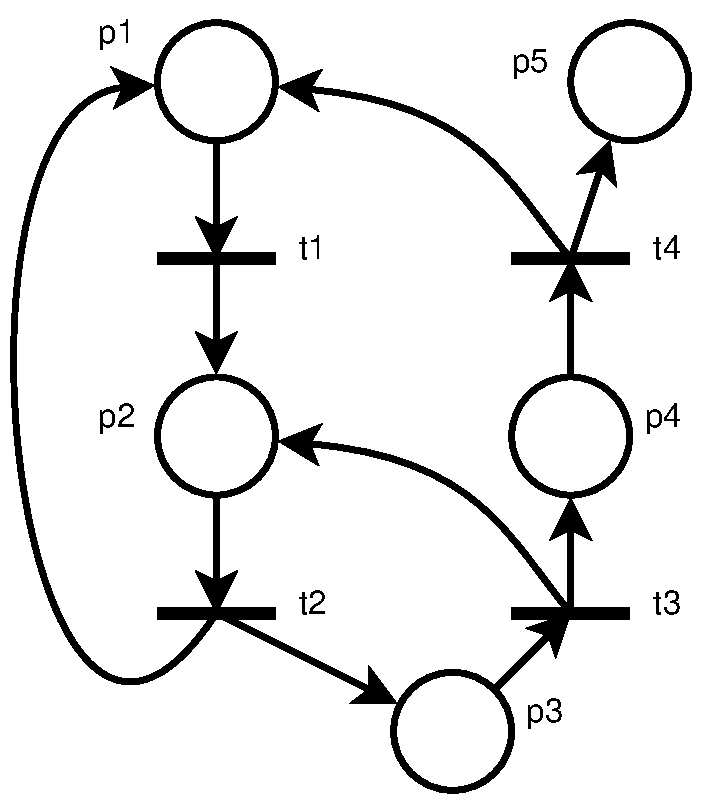
\includegraphics[width=0.3\textwidth]{Figures/EleccionSubredZonasInfluencia_1.eps}\end{matrix}
  \ \ \ \equiv \ \ \ 
 \begin{matrix}  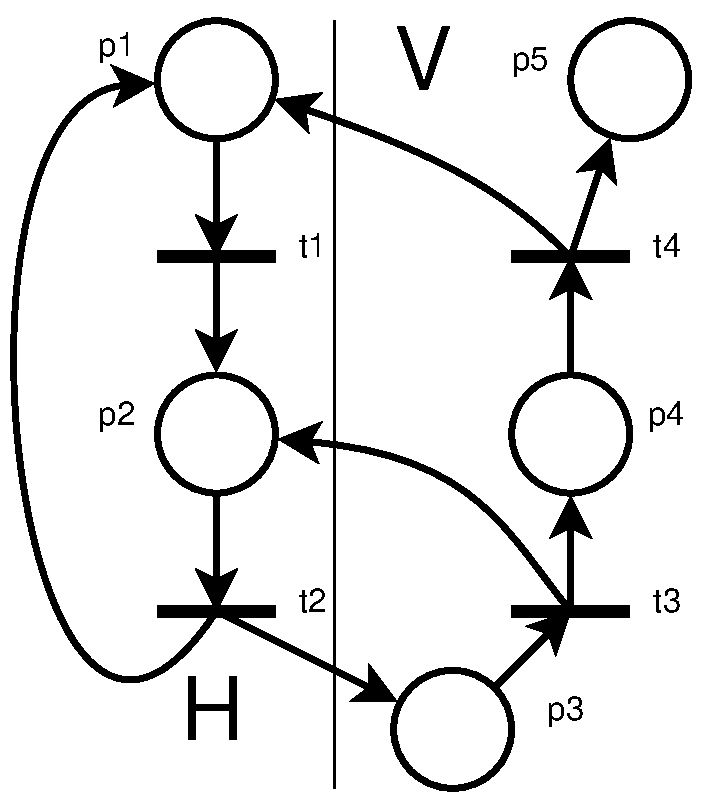
\includegraphics[width=0.3\textwidth]{Figures/EleccionSubredZonasInfluencia_2.eps}\end{matrix}
\]
\rule{35em}{0.5pt}
 \caption{Selecting subnet to hide}
 \label{fig:seleccion_subred_oculta} 
\end{figure}



\begin{example}
Consider the Petri net of the figure \ref{fig:seleccion_subred_oculta} with the next incidence matrix:
\[
\kbordermatrix{
   & t_1 & t_2 & t_3 & t_4\\
p_1& -1 &  1  &  0  &  1 \\
p_2&  1 & -1  &  1  &  0 \\
p_3&  0 &  1  & -1  &  0 \\
p_4&  0 &  0  &  1  & -1 \\
p_5&  0 &  0  &  0  &  1 \\
}
\]


The subnet we want to hide is formed by places $p_1$ and $p_2$ and transitions
$t_1$ and $t_2$. Graphically, separate places and transitions to hide (H) from the rest of the network (V)

The incidence matrix is already sorted by the places and transitions to the top of it. Here are the four parts described above.
\[
\kbordermatrix{
   & t_1& t_2 & \vline &t_3 & t_4\\
p_1& -1 &  1  & \vline &  0  &  1 \\
p_2&  1 & -1  & \vline &  1  &  0 \\
\hline
p_3&  0 &  1  & \vline & -1  &  0 \\
p_4&  0 &  0  & \vline &  1  & -1 \\
p_5&  0 &  0  & \vline &  0  &  1 \\
}
\]

In this matrix we can see:
\begin{itemize}
  \item $H=\kbordermatrix{ & t_1 & t_2\\ p_1 & -1 & 1\\p_2 & 1 & -1\\}$
        is the subnet we want to hide. It is the same as $N_1$
  \item $V=\kbordermatrix{&t_3&t_4\\p_3&-1&0\\p_4&1&-1\\p_5&0&1\\}$ is the
        subnet that is visible. It is the same as $N_2$
  \item $HP=\kbordermatrix{ & t_3 & t_4\\ p_1 & 0 & 1\\p_2 & 1 & 0\\}$ are
        the relationships between transitions of V and H places. It is the
        equivalent to $PIM_1$ or $TIM_2$
  \item $HT=\kbordermatrix{&t_1&t_2\\p_3&0&1\\p_4&0&0\\p_5&0&0\\}$ are
        the relationships between places of V and H transitions. It is the
        equivalent to $TIM_1$ or $PIM_2$
\end{itemize}
\end{example}

At this moment, it is easy to see that we can choose any subset of places
and transitions in order to hide it, simply reordering rows and columns.

\begin{example}
In the previous example we have seen a fairly simple option selection
subnet and we have chosen the place $p_1$ and $p_2$ and transitions $t_1$
and $t_2$. However, we can choose any other subset of places and transitions.
In this example we will select places $p_2$, $p_3$ and $p_5$ and the transitions
$t_1$ and $t_3$. Thus, in the graph of the previous example move the locations and transitions to hide on one side and the rest on the other.
\begin{center}
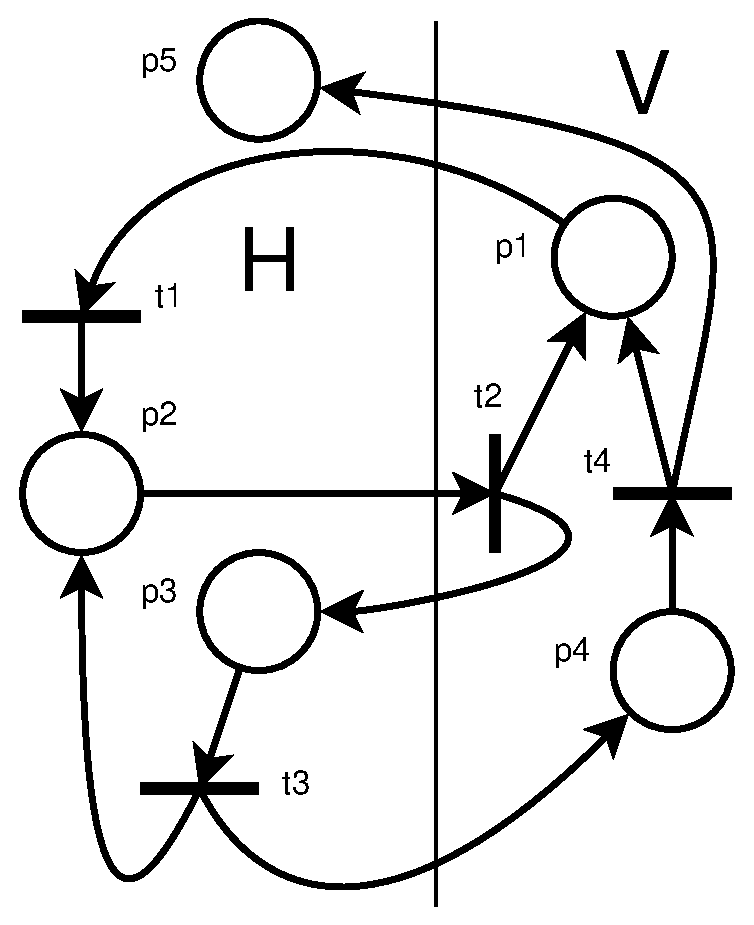
\includegraphics[width=0.3\textwidth]{Figures/EleccionSubredZonasInfluencia_3.eps}
\end{center}
Although more confusing, can be seen that the graph is the same as the incidence matrix is the same (not just part of the equivalence class, it is exactly the same). Now, in this matrix move places $p_2$, $p_3$ and $p_5$, and transitions $t_1$ and $t_3$ at the beginning of the matrix:
\[
\kbordermatrix{
   & t_1& t_3 & \vline &t_2 & t_4\\
p_2&  1 &  1  & \vline & -1  &  0 \\
p_3&  0 & -1  & \vline &  1  &  0 \\
p_5&  0 &  0  & \vline &  0  &  1 \\
\hline
p_1& -1 &  0  & \vline &  1  &  1 \\
p_4&  0 &  1  & \vline &  0  & -1 \\
}
\]

Interpreting each of the chunks of the matrix is similar to the previous example.
\end{example}


\subsection{Front-end interaction with the subnet. Input and output functions}

Once you have defined all this environment, we will try to go a little further.
Let's assume that we want to export a subnet we have hidden in another network,
like a black box. Our intention is to connect this hidden network to another
network, and can thus be reused subnets. For example, let's assume that we
have a process modeling with Petri net modeling and in this there is a subnet
we want to hide, but, at the same time, we want to reuse it in other Petri
nets.

In this case we have a problem, and once hidden network disappears half the
information input or output arcs of the same. In particular, we do not know
the source nodes and arcs that leave the target nodes of the arcs that enter
the network until no visible again. But if we want to reuse it on other networks,
can not wait to make it visible. Should remain hidden, but should be able
to connect to other networks.

We will try to solve this problem. This way we can reuse hidden networks
like plug-in modules on other networks. However, we will not need the actual
implementation of the source or destination nodes of the arcs that leave
or enter the network, respectively. The solution is to define a facade or
front-end input and output of the network. This front-end will contain the
information needed to interact with the network hidden, but hide the specifics
of implementation. To define this behavior going from some assumptions.

\subsubsection{Previous definitions}

Let $N=\langle P,T,\alpha,\beta\rangle$ be a Petri net and let $P=\{N_1,
N_2\}$ be a partition of $N$. 

\begin{definition}[Input place]
Let $p_i$ a place of $N_1$. $p_i$ is an input place of $N_1$ if it is the
destination of an arc coming from a $N_2$ transition, ie,
\[
p_i \mbox{ is an input place of } N_1 \mbox{ if } \exists t_j \in N_2\ |
c_{ij}>0
\]
\end{definition}

\begin{definition}[Input transition]
Let $t_i$ a transition of $N_1$. $t_i$ is an input transition of $N_1$ if
it is the destination of an arc coming from a $N_2$ place, ie,
\[
t_i \mbox{ is an input transition of } N_1 \mbox{ if } \exists p_j \in N_2
| c_{ji}<0
\]
\end{definition}

\begin{definition}[Input node]
An input node of $N_1$ is an input place or transition of $N_1$.
\end{definition}

\begin{definition}[Output place]
Let $p_i$ be a place of $N_1$. $p_i$ is an output place of $N_1$
if an arc leaves it towards a transition of $N_2$, ie,
\[
p_i \mbox{is an output place of } N_1 \mbox{ if } \exists t_j \in N_2 | c_{ij}
< 0
\]
\end{definition}

\begin{definition}[Output transition]
let $t_i$ be a transition of $N_1$. $t_i$ is an output transition of $N_1$
if an arc leaves it towards a place of $N_2$, ie,
\[
t_i \mbox{ is an output transition of } N_1 \mbox{ if } \exists p_j \in N_2
| c_{ji} > 0
\]
\end{definition}

\begin{definition}[Output node]
An output node of $N_1$ is an output place or transition of $N_1$.
\end{definition}

After defining these concepts, we can define the sets thereof.

\begin{notation}
We denote the sets of the elements defined above:
 \begin{shortitemize}
  \item Let $IP(N) \subseteq  \overline P$ (Input Places) be the set of input
   places of a subnet.
  \item Let $IT(N) \subseteq \overline T$ (Input Transitions) be the set
   of input transitions of a subnet.
  \item Let $IN(N) \subseteq \overline P \cup \overline T$ (Input Nodes)
        be the set of input nodes of a subnet.
  \item Let $OP(N) \subseteq  \overline P$ (Output Places) the set of output
        places of a subnet.
  \item Let $OT(N) \subseteq \overline T$ (Output Transitions) be the set
        of output transitions of a subnet.
  \item Let $ON(N) \subseteq \overline P \cup \overline T$ (Output Nodes)
        be the set of output nodes of a subnet.
\end{shortitemize}
\end{notation}

\begin{note}
Recall that a node in a Petri net can be both a place and a transition, depending
on the context.
\end{note}
\begin{notation}
Denote as $ n_i $ to a node of a Petri net.
\end{notation}

\begin{figure}[htbp]
\centering
\[
 \begin{matrix} 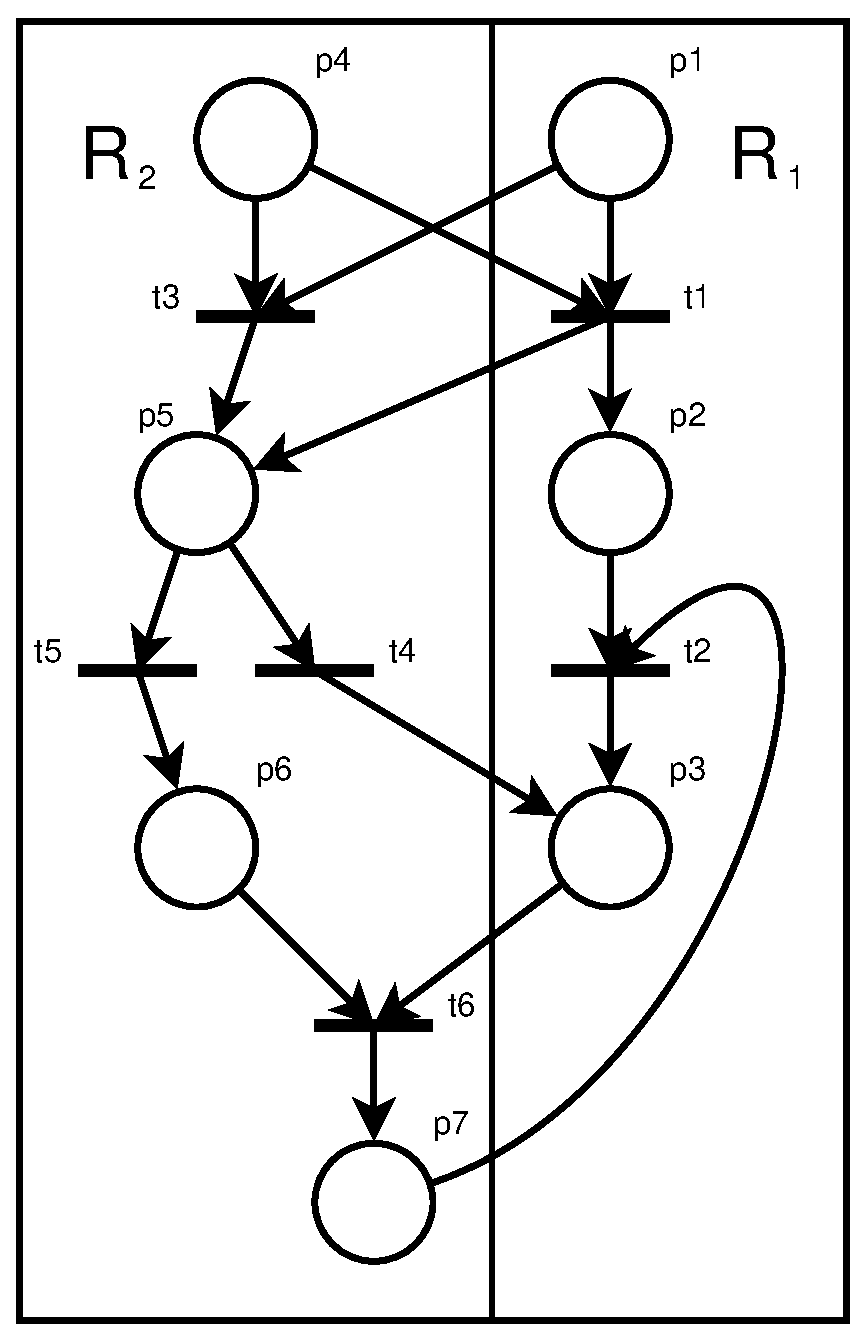
\includegraphics[width=0.4\textwidth]{Figures/NodosEntradaSalidaV.eps}\end{matrix}
  \ \ \ \ \ 
C=
\kbordermatrix{
   & t_1 & t_2 & \vline & t_3 & t_4 & t_5 & t_6\\
p_1& -1 &  0  &  \vline & -1  &  0 & 0  &  0 \\
p_2&  1 & -1  &  \vline & 0  &  0 & 0  &  0 \\
p_3&  0 &  1  &  \vline & 0 &  2 & 0  &  -1 \\
\hline
p_4&  -1 &  0  &  \vline & -1  & 0 & 0  &  0 \\
p_5&  2 &  0  &  \vline & 1  &  -1 & -1  &  0 \\
p_6&  0 &  0  &  \vline & 0  &  0 & 1  &  -1 \\
p_7&  0 &  -3  &  \vline & 0  &  0 & 0  &  1 \\
}
\]
\rule{35em}{0.5pt}
\caption{Subnets with input and output nodes}
\label{fig:nodos_entrada_salida} 
\end{figure}


As we have generic definitions, no problem in applying to a network divided
into $ H $, $ V $, $ HN $ and $ HT $, as the set $ \{H, V \} $ is a partition
of $ N $.

\subsubsection{Subnet Front-end}

Once all these concepts, we create the front-end input/output of a Petri subnet. A front-end of the Petri net will be a intermediate facade that allows us to physically divide that subnet from the rest of the net. Thus, in order to enter or leave the subnet, you need to make it through this front-end.

Let $ IA $ (input arcs) the set of arcs that enter the subnet $ N_1 $ and let $ OA $ (output arcs) the set of arcs leaving $ N_1 $.

\begin{definition}[Input gate of a net]
Let $ a_i \in IA $ an arc of entrance to $ N_1 $. We define an input gate to $ N_1 $, and denote by $ ig_i $, as a new logical node that is identified with an arc of entrance to the net. For each input arc, defines an input gate with
the same weight, regardless of the origin and destination of the arc. If the source is a transition, we denote $ igt_i $ and if a place, $ igp_i $.
\end{definition}

\begin{definition}[Output gate of a net]
Let $ a_i \in OA $ output arc $ N_1 $. We define an output gate of $ N_1 $, and denote by $ og_i $, as a new logical node that is identified with an exit arc of the net. For each exit arc is defined an output gate with
the same weight, regardless of the origin and destination of the arc. If the source is a transition, we denote $ ogt_i $ and if it is a place, $ ogp_i$.
\end{definition}

In this way we can divide the input arcs and output into two parts: a $ N_1 $ internal and external to $ N_1 $. If we take an arc of entrance $ a_i $ that has an origin in $n_j $ and destination
in $ n_k $, we define an input gate through a point of entry so that the original arc $ a_i $ is divided into two parts.
\begin{itemize}
  \item $a_{i1}$ (external to $N_1$) with origin in $n_j$ and destination  in $igt_i$ or $igp_i$ depending on if $n_j$ is a transition or a place,
and the same weight as the input gate.
  \item $a_{i2}$ (internal to $N_1$) with destination in $igt_i$ or $igp_i$ depending on if $n_j$ is a transition or a place respectively,
and the same weight as the input gate.
\end{itemize}

Similarly, if we take an exit arc $ a_i $ that has an origin in $ n_k $ and destination in $ n_j $, we define an output gate $ og_i $ so that the original arc $ a_i $ is divided into two parts:
\begin{itemize}
  \item $a_{i1}$ (internal to $N_1$) with origin in $n_k$ and destination
  in $ogt_i$ or $ogt_i$ depending on if $n_j$ is a transition or a place,
and the same weight as the output gate.
  \item $a_{i2}$ (external to $N_1$) with destination in $n_j$ and origin
  in $igt_i$ or $igp_i$ depending on if $n_j$ is a transition or a place
  respectively,
and the same weight as the output gate. 
\end{itemize}

\begin{example}
\label{ej:puertas_entrada_salida}
Consider the net in figure \ref{fig:nodos_entrada_salida}. In this network we have three arcs entering and three arcs leaving. For each of those that
leave, I define output gates and for each coming one, we define input gates. The weight of each gate (if it is different than 1) is placed in a little square inside. The subnet $ N_1 $ becomes:
\[
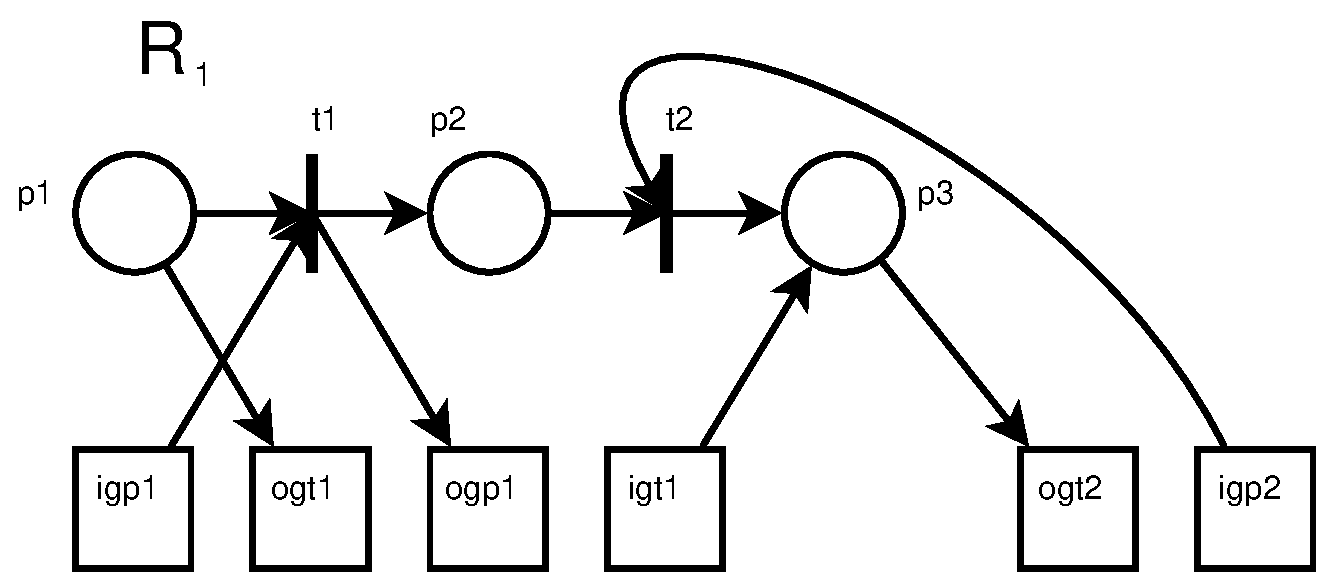
\includegraphics[width=0.7\textwidth]{Figures/PuertasEntradaSalida_1.eps}
\]
and in the complete net, arcs entering and leaving are divided into two pieces:
\[
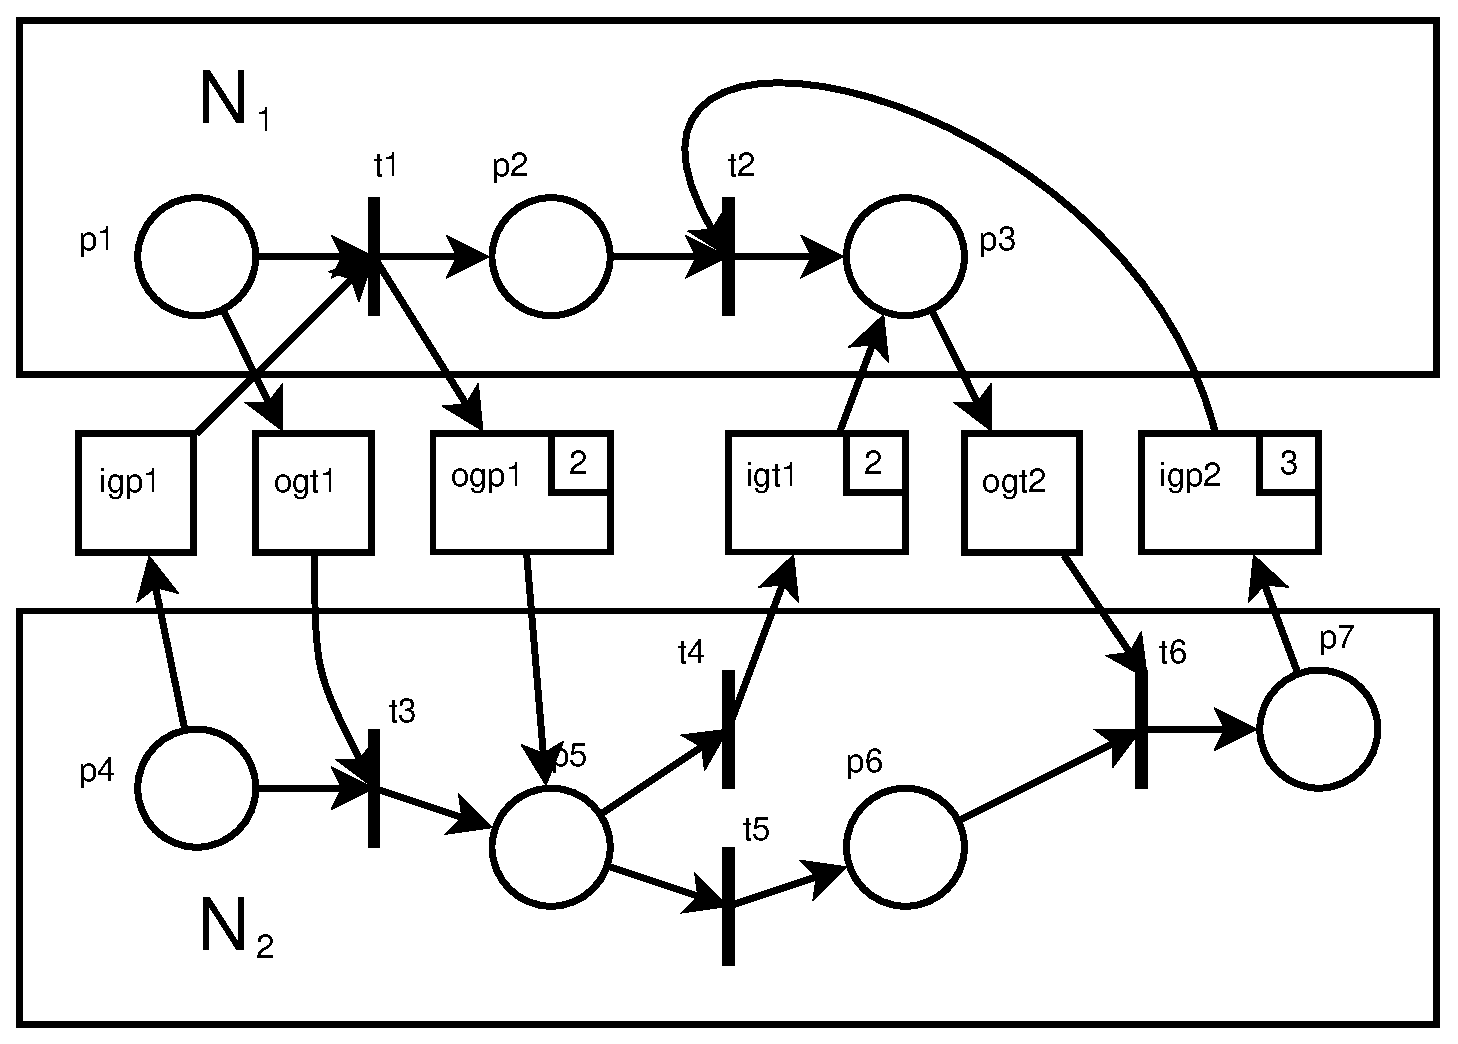
\includegraphics[width=0.7\textwidth]{Figures/PuertasEntradaSalida_2.eps}
\]
\end{example}

\begin{definition}[Input Front-end of a net]
The input front-end (or input interface) of a subnet $N_1$ is the set of all input gates of $ N_1 $. We denote by $ IF $ of $ N_1 $.
\end{definition}

\begin{definition}[Output Front-end of a net]
The output front-end (or output interface)of a subnet $N_1$ is the set of all output gates of $ N_1 $. We denote by $ OF $ of $ N_1 $.
\end{definition}

\begin{definition}[Front-end of a net]
The front-end (or interface) of a net $N_1$ is the pair of $IF$ and $OF$ of $N_1$. We denote by $ F $ of $ N_1 $.
\[
F = \langle IF, OF\rangle
\]
\end{definition}

\begin{example}
Taking the net of the example \ref{ej:puertas_entrada_salida} and applying these new definitions, we would have $ N_1 $ net along with its front end as shown in Figure \ref{fig:front-end}.
\end{example}

\begin{figure}[htbp]
\centering
\[
 \begin{matrix} 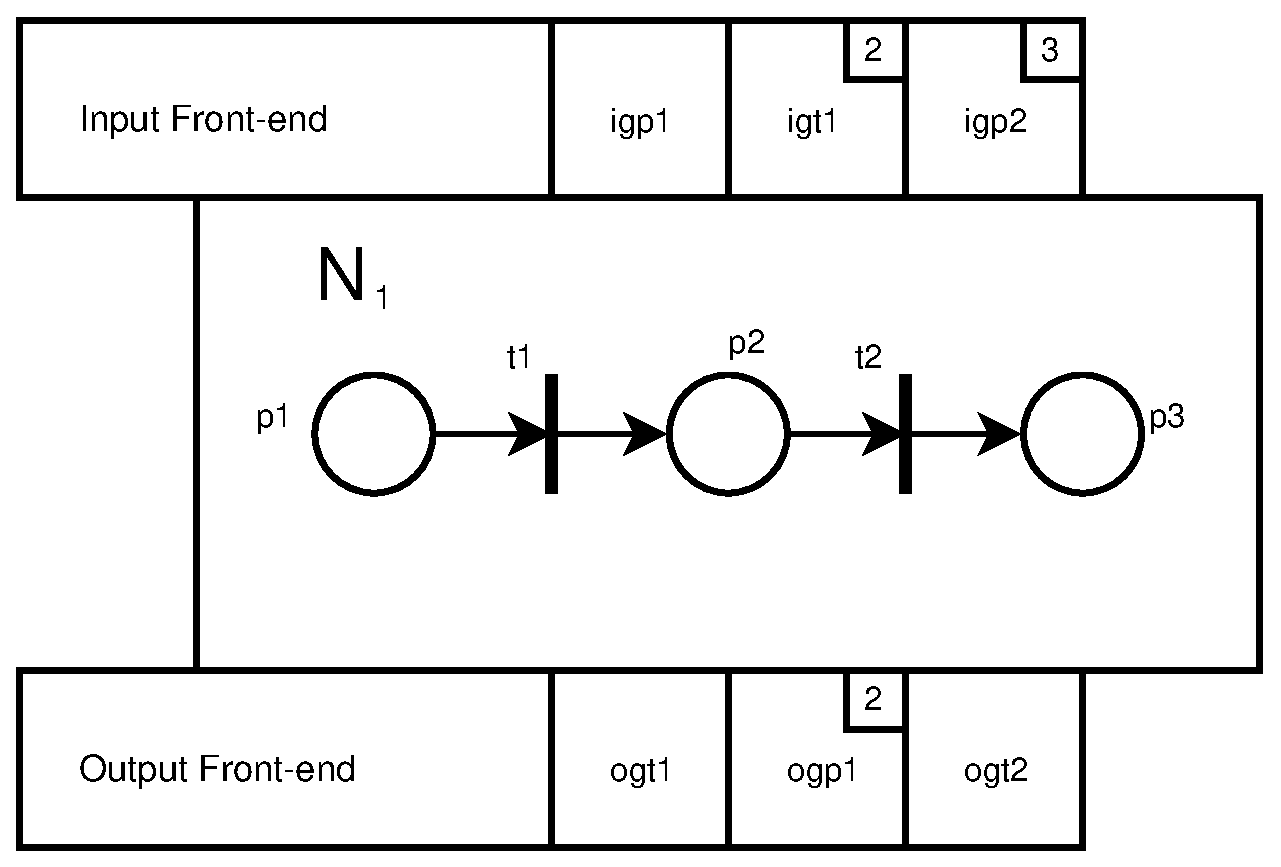
\includegraphics[width=0.6\textwidth]{Figures/Front-endEnglish.eps}\end{matrix}
\]
\rule{35em}{0.5pt}
 \caption{Front-end of a net}
 \label{fig:front-end} 
\end{figure}


\subsubsection{Input/output functions}

Once all these input and output concepts defined, we will introduce a few key concepts for our purpose.

Let $ N $ a Petri net and let $ \{N_1, N_2 \} $ a partition of $ N $. Let $ F = \langle IF, OF \rangle $ the front-end of $ N_1 $.

\begin{definition}[Petri net Input function]
 We define the input function $f_i$ of $N_1$ as:
\[
  f_i:F \longrightarrow IN
\]
such that for each input gate $ igt_i$ you mapped one or no input place $ N_1 $ and each input gate $ igp_j$ you mapped one or no input transition $ N_1 $. 

\end{definition}

\begin{definition}[Petri net Output function]
We define the output function $f_o$ of $N_1$ as:
\[
  f_o:ON \longrightarrow F
\]
such that each output place $ N_1 $ you mapped one or no output gate $ ogt_i $ of $ N_1 $ and each output transition $ N_1 $ you mapped one or no output gate $ ogp_j $ to $ N_1$
\end{definition}

The input function can be defined for all the input gates and the output function should be surjective because if not, some door would not be connected. Anyway that is not essential. If a front-end door is not connected with any element of your network, simply by solving the final network, the arcs connected to that door disappear. Note also that the input function is not necessarily injective: Multiple input gates can be associated to the same node of $ N_1 $.

\begin{example}
Consider the net $ N_1 $ in figure \ref{fig:nodos_entrada_salida} with its front-end in figure \ref{fig:front-end}. The input and output functions are:

\begin{itemize}
\item Input function: 
$
\begin{array}{c|ccc}
F & igp_1 & igt_1 & igp_2\\
\hline
IN & t_1 & p_3 & t_2\\
\end{array}
$
\item Output function: 
$
\begin{array}{c|ccc}
ON & p_1 & t_1 & p_3\\
\hline
F & ogt_1 & ogp_1 & ogt_2\\
\end{array}
$
\end{itemize}
\end{example}

\subsubsection{Attachable net}

By joining the subnet $ R_1 $ along with its front-end and its input and output functions $ f_i $ and $ f_o $ we grouped both the internal network with external communication. This way we can ''extract'' a subnet and ''implant'' it in another net. You only need this destination network is to communicate with the front-end. So naturally appears the following definition.

\begin{definition}[Attachable Petri net]
An Attachable Petri net is a quadruple $R_a=\langle R,F,f_i,f_o\rangle$
\end{definition}

From these definitions, it is clear that you can create attachable subnets taking a subnet of another given and applying the whole process we have defined. But it is also possible to create from scratch, starting from a network, defining a front end for that network and declaring the input and output functions. So you can create Petri nets modules providing functionality and out through a front-end without requiring the actual implementation.

\begin{example}
The attachable net in figure \ref{fig:nodos_entrada_salida} would be the
next:
\[
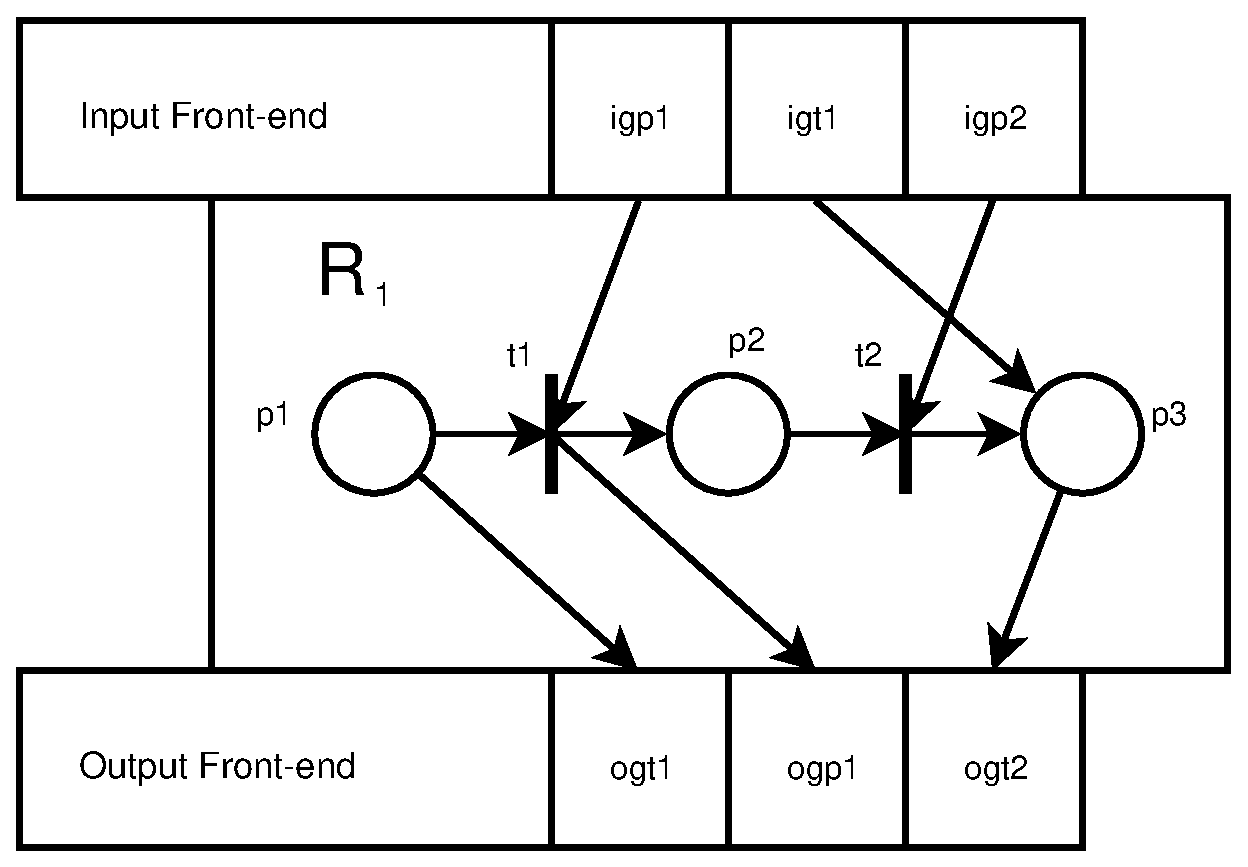
\includegraphics[width=0.6\textwidth]{Figures/RedAcoplable_1English.eps}
\]
\end{example}
It can be seen as a private black box with visible input and output connectors that are ''plugged'' to other networks. In a attachable net, the private part would be $ N_1 $, $ f_i $ and $ f_o $. The public part of the front-end would be $ F $. All a net need to know is the input/output front-end.

A utility of these nets is that its definition is simple, since only the front-end is needed to define its operation. This makes possible to create nets using attachable nets in certain areas where they do not know their actual implementation, but its behavior. Additionally, it is possible to use different implementations of ''network providers'' of the same attachable nets, using at each moment the most appropriate one.

\begin{example}
Consider now the following Petri net
\[
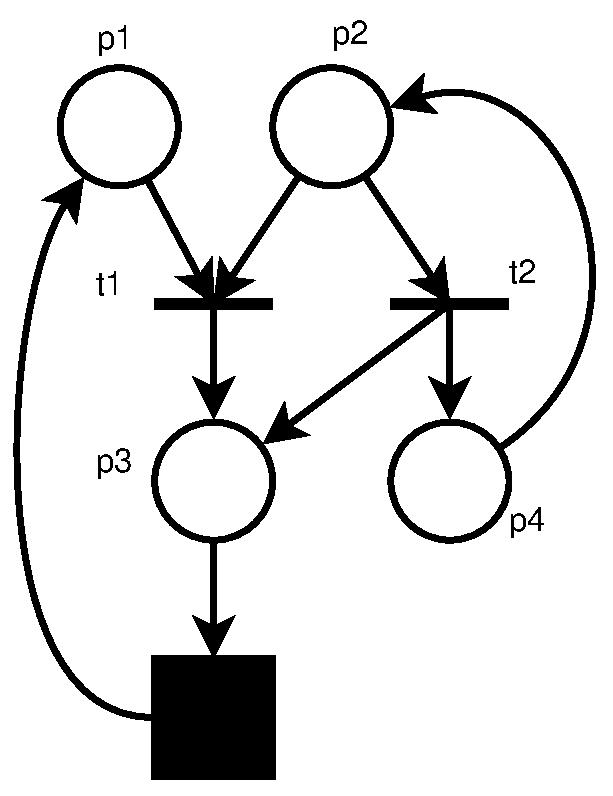
\includegraphics[width=0.3\textwidth]{Figures/RedAcoplable_2.eps}
\]
to which we want to connect an attachable net in the black box. Let's assume we have two equivalent alternatives described in Example \ref{ej:ocultacion_reduccion}:
\[
 \begin{matrix} 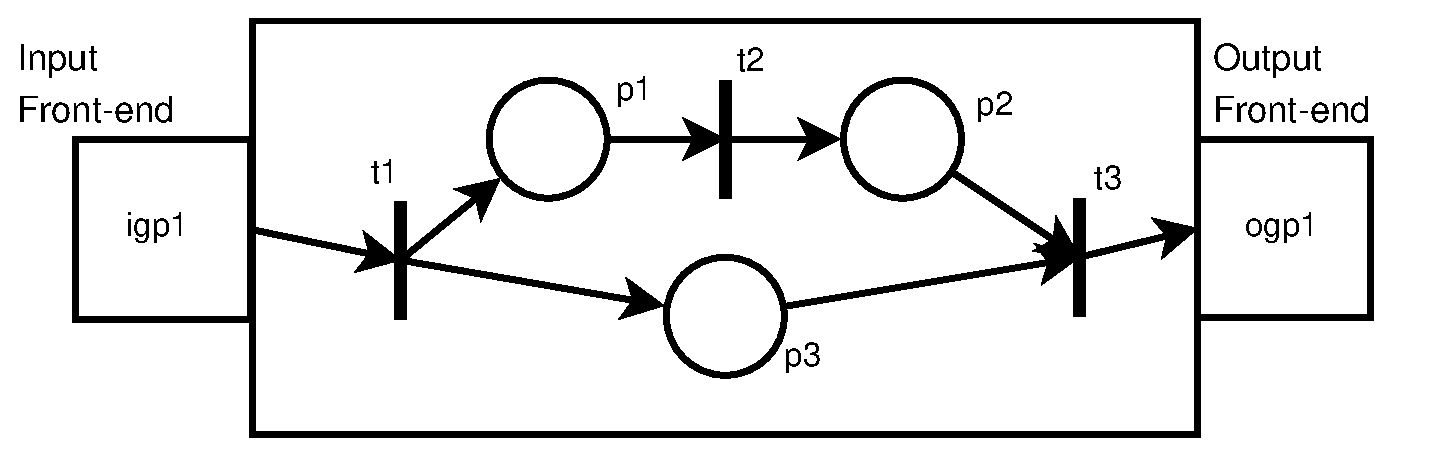
\includegraphics[width=0.6\textwidth]{Figures/RedProveedor_1English.eps}\end{matrix}
\]
\[
 \begin{matrix}  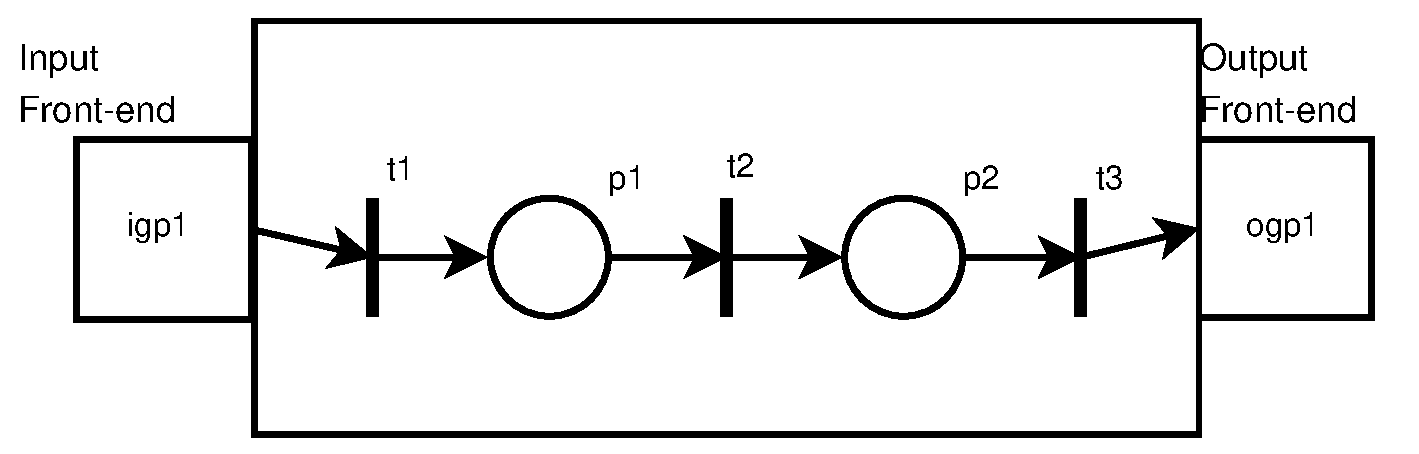
\includegraphics[width=0.6\textwidth]{Figures/RedProveedor_2English.eps}\end{matrix}
\]

We Can ''plug'' either because their front ends are equivalent and remains in figure \ref{fig:redes_acoplables}.



\begin{figure*}[htbp]
\centering
\[
 a) \ \ 
 \begin{matrix} 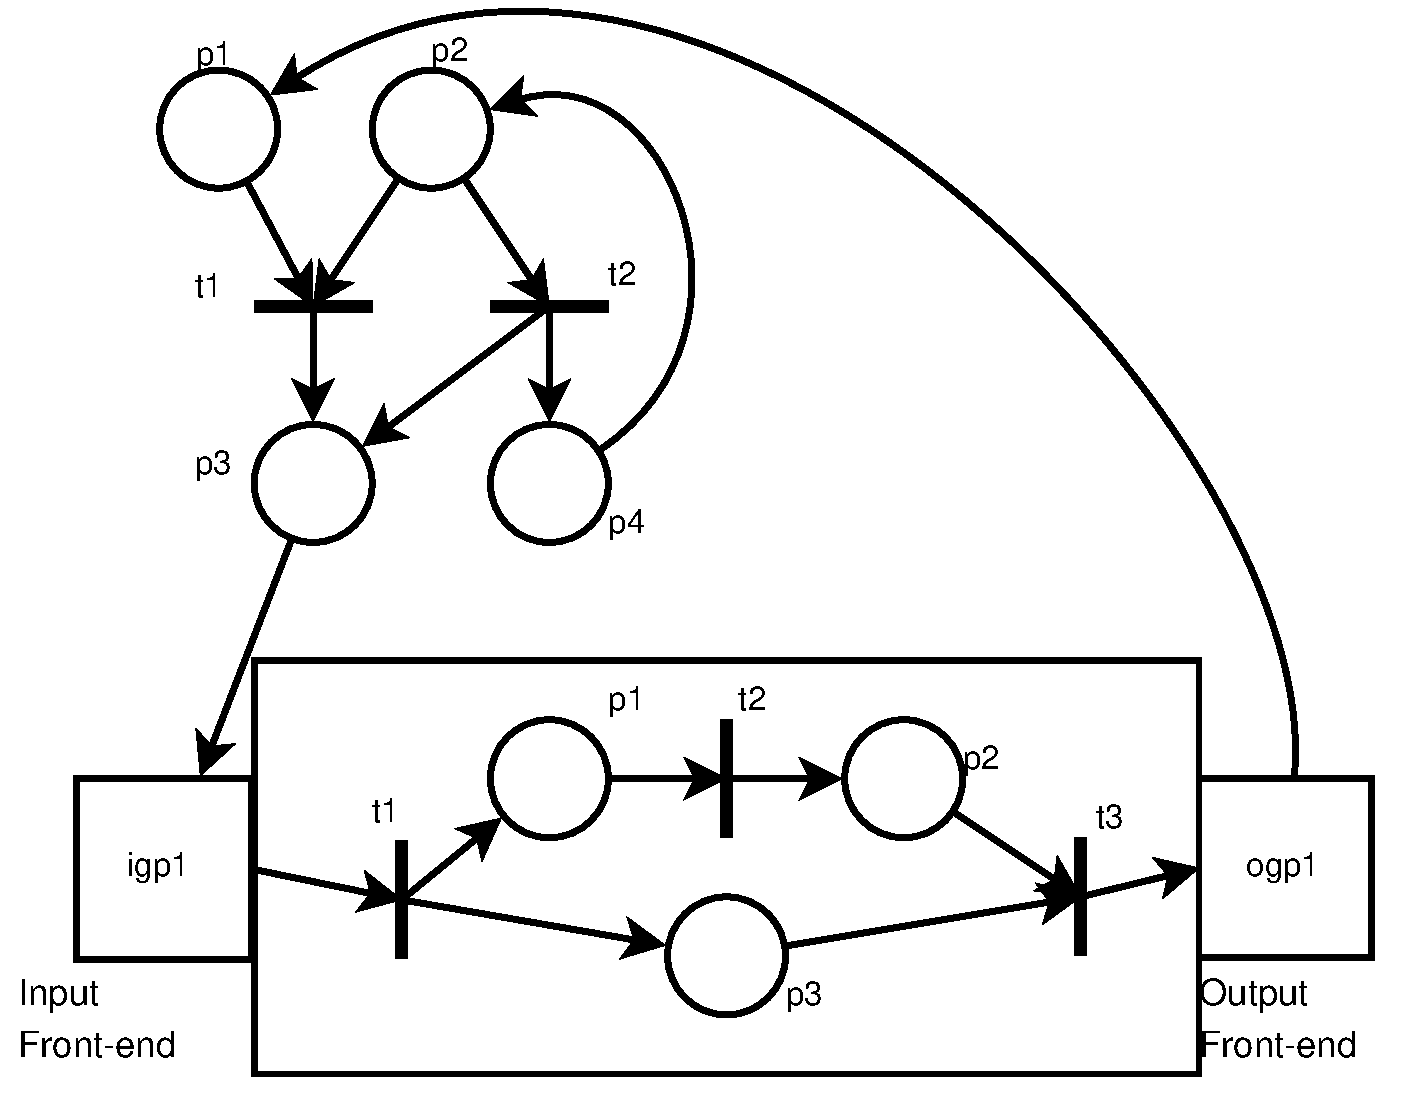
\includegraphics[width=0.4\textwidth]{Figures/RedAcoplableProveedor_1English.eps}\end{matrix}
 b) \ \ 
 \begin{matrix}  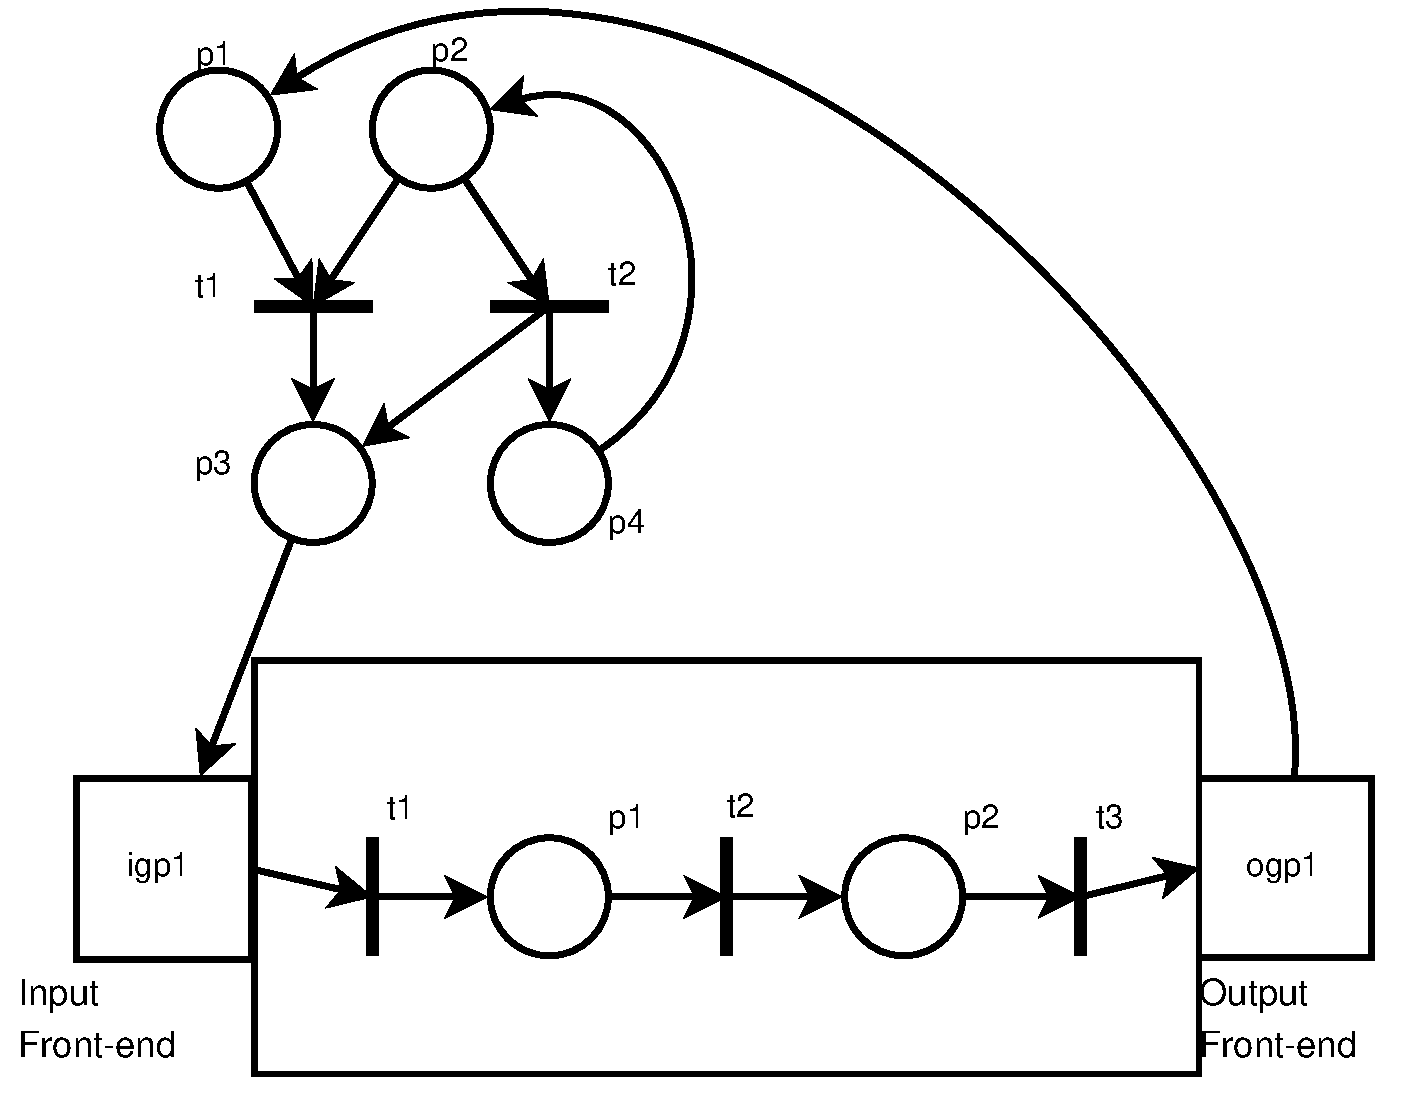
\includegraphics[width=0.4\textwidth]{Figures/RedAcoplableProveedor_2English.eps}\end{matrix}
\]
\rule{35em}{0.5pt}
\caption{Two different implementations of attachable nets}
\label{fig:redes_acoplables}
\end{figure*}
In this case, the behavior of the net will be the same, but does not have to be. That will decide who connects nets. For example, you could create a ''foo'' net that does nothing at first and replace it later by the real
one.
\end{example}

\section{Private information. Hiding a subnet}

Once we have defined subnets and front-ends we can select one of them to
securize it by hiding. We proceed to the occultation
as such \cite{HID-Inigo2011MT}. Graphically, it seems simple. Just replace the subnet to hide by a black box and modify some arcs according to the following
rules:

\begin{enumerate}
\item The arcs originating in a place or transition within the black box, and target a place or transition out of it will have the black box as the source.
\item The arcs originating in a place or transition out of the black box, and target a place or transition within it, are replaced by the black box as a destination.
\end{enumerate}

\begin{example}
We consider the Petri net of the  Figure \ref{fig:seleccion_subred_oculta}.
The result of hiding the part of the graph H is the following:
\[
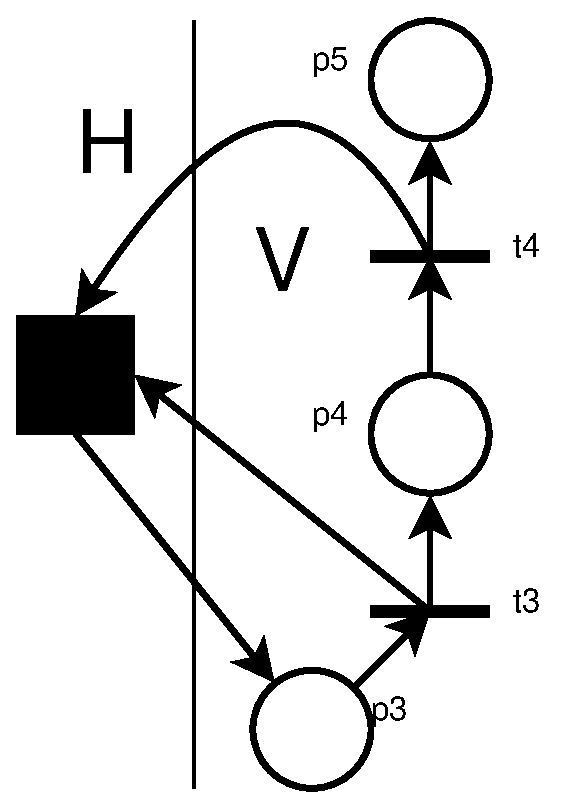
\includegraphics[width=0.3\textwidth]{Figures/OcultacionSubred_1.eps}
\]
\end{example}

In the associated incidence matrix also replace the H elements by a black box:
\[
\kbordermatrix{
   & t_1 &  t_2 & \vline &t_3 & t_4\\
p_1& \rule{0.15in}{0.15in} & \rule{0.15in}{0.15in}    & \vline &  0  &  1 \\
p_2& \rule{0.15in}{0.15in} & \rule{0.15in}{0.15in}   & \vline &  1  &  0 \\
\hline
p_3&  0 &  1  & \vline & -1  &  0 \\
p_4&  0 &  0  & \vline &  1  & -1 \\
p_5&  0 &  0  & \vline &  0  &  1 \\
}
\]

However, in this matrix notation is given information should also be hidden: it gives us information about the number of places and transitions of the hidden subnet, besides indicating hidden places and transitions with which it interacts. To solve this problem we proceed as follows. We can group all rows for the screened subnet into one. In each row position examine all elements of the original rows corresponding to that position, and will put:

\begin{itemize}
\item If all these elements are zero, in the grouped row will be a zero.
\item If one and only one of those elements is nonzero, will put that item.
\item If there are several non-zero elements, we will post a list of these items separated by commas, creating a d-dimensional element (in $ d $ dimensions).
\end{itemize}

In the same way we have done with the rows, proceed with columns. Thus, if the hidden subnet has $ i $ columns and $ j $ rows, we will get a matrix
like this:
\[
\left(
\begin{array}{c|ccc}
 \rule{0.15in}{0.15in} & a_{1(i+1)} & \cdots & a_{1m} \\
 \cline{1-4} 
 a_{(j+1)1} & &   & \\
 \vdots & & V & \\
 a_{n1} & &   & \\
\end{array}
\right)
\]

where $\forall p, \forall q |  i+1\le p \le m \land j+1\le q \le n$
\[
a_{1p}=\left\{ \begin{array}{ll}
0 & \mbox{ if }\forall r | 1 \le r \le j, c_{rp}=0\\
c_{rp}& \mbox{ if } \exists! r, 1 \le r \le j | c_{rp}\neq0\\
(c_{r_1p}, c_{r_2p},...) & \mbox{ if }\exists r_1\neq r_2 \neq ..., 1 \le r_1, r_2,... \le j |c_{r_1p},c_{r_2p},...\neq0
\end{array}\right.
\]

\[
a_{q1}=\left\{ \begin{array}{ll}
0 & \mbox{ if }\forall s | 1 \le s \le i, c_{qs}=0\\
c_{qs}& \mbox{ if } \exists! s, 1 \le s \le i | c_{qs}\neq0\\
(c_{qs_1}, c_{qs_2},...) & \mbox{ if }\exists s_1\neq s_2 \neq ..., 1 \le s_1, s_2,... \le s |c_{qs_1},c_{qs_2},...\neq 0
\end{array}\right.
\]

So we hide the number of places and transitions of the hidden subnet
and their relationships.
Yes, some information is given about the hidden network. Really if this resulting matrix some node that is d-dimensional, at least in the hidden network must exist $ d $ nodes of this type.

Furthermore, each nonzero element define part of the front-end of the
subnet. If we take the elements of the first row (the first element of the column
is the hidden subnet):
\begin{itemize}
\item any element greater than zero defines an $ogt$ towards the transition
related by the column
\item any element less than zero defines an $igt$ from the transition related
by the column
\end{itemize}

If we take the elements of the first column (the first element of the column
is the hidden subnet):

\begin{itemize}
\item any element greater than zero defines an $igp$ towards the place
related by the row
\item any element less than zero defines an $ogp$ from the place related
by the row
\end{itemize}

With this information we can build the entire front-end of the subnet.

\begin{example}
We consider the Petri net defined by the following incidence matrix, separated into $H$,$V$,$HT$ and $HP$.
\[
\kbordermatrix{
   & t_1 & t_{2} & t_{3} & \vline & t_{4} & t_{5} & t_{6}\\
p_1 & -1 & 0 & 1 & \vline & 0 & 0 & 0\\
p_2 & -1 & 0 & 0 & \vline & 1 & 0 & 1\\
p_3 & 1 & 0 & 0 & \vline & -1 & 0 & 0\\
p_4 & 1 & -1 & 0 & \vline & 2 & 0 & 0\\
\hline
p_5 & 0 & 1 & 0 & \vline & 0 & 0 & 0\\
p_6 & 3 & 0 & -1 & \vline & 0 & 0 & 0\\
p_7 & 0 & 0 & 0 & \vline & -1 & -1 & 1\\
p_8 & 0 & 0 & 0 & \vline & 0 & 1 & -1\\
}

\]

After applying the above steps for the group, we would have the following:
\[
\kbordermatrix{
&   & \vline& t_4 & t_5 & t_6\\
&\rule{0.15in}{0.15in} & \vline& (1,-1,2) & 0 & 1\\
\hline
p_5 & 1  & \vline& 0 & 0 & 0\\
p_6 & (3,-1) & \vline& 0 & 0 & 0\\
p_7 & 0 & \vline&  -1 & -1 & 1\\
p_8 & 0 & \vline&  0 & 1 & -1\\
}
\]

Here we see that the information about the number of hidden places and transitions is minimized. So we know that at least there are two hidden transitions and at least three hidden places (there is a transition of dimension 3). However, we do not know the exact number of either. 

Now we can build the front-end. The elements of the first row are $(1,-1,2)$
and $1$. So we have three $ogt$ and one $igt$. The elements of the first
column are $1$ and $(3,-1)$, so defines two $igp$ and one $ogp$ like this.
This is the subnet front-end, having hidden its inner content.

\[
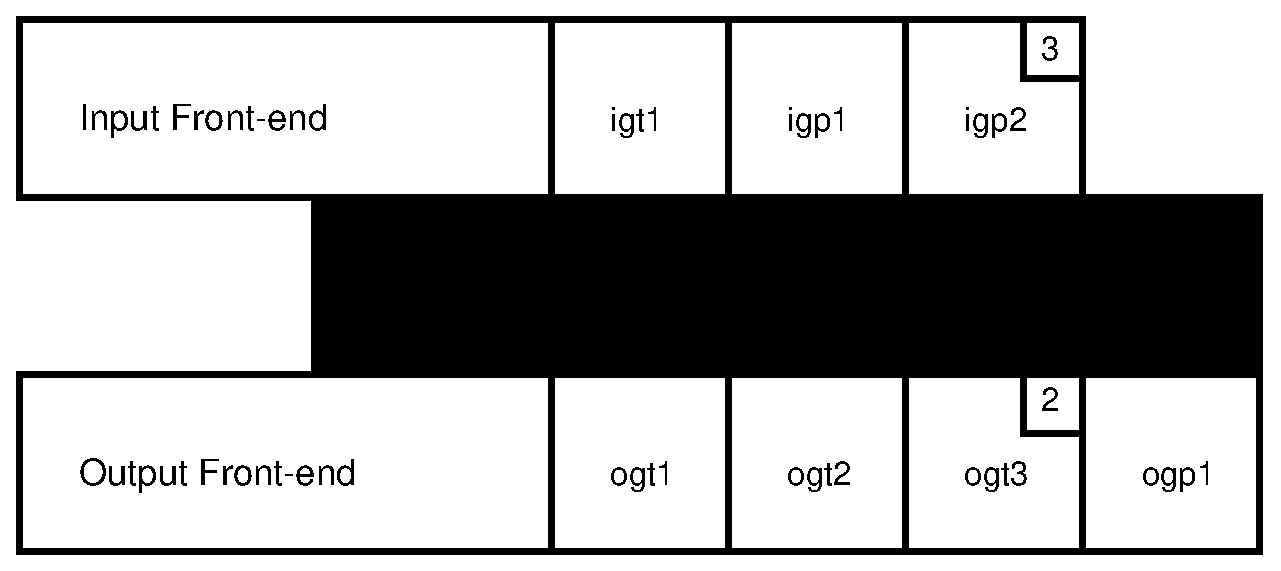
\includegraphics[width=0.6\textwidth]{Figures/frontendSubredOculta.eps}
\]

\end{example}




\subsection{Hiding vs. Reduction}

Both Silva works \cite{G-Silva1985,SM-Silva19931} as in the article by Xia \cite{R-Xia20111662} discusses possible Petri nets reductions for grouping and simplifying, under certain circumstances, places and/or transitions. These reductions can be structural (only dependent on the structure and initial marking of the net) or depending on the interpretation of the Petri net.

Should be clear that these reductions are not the same thing we are describing. We do not try to simplify the network together elements to have more or fewer places or transitions or to make it easier. What we want is to hide part of the network, regardless of how simple or complicated it is.

Here we have an example of what a reduction is.

\begin{example}[Reduction of an implicit place \cite{G-Silva1985}]
\label{ej:ocultacion_reduccion}
In a marked Petri net, an implicit place is one that meets the following:
\begin{shortenumerate}
 \item its marking can be calculated from other points marking
 \item never is the only place that prevents the enabling of its output transitions
\end{shortenumerate}
If we consider the following Petri net
\[
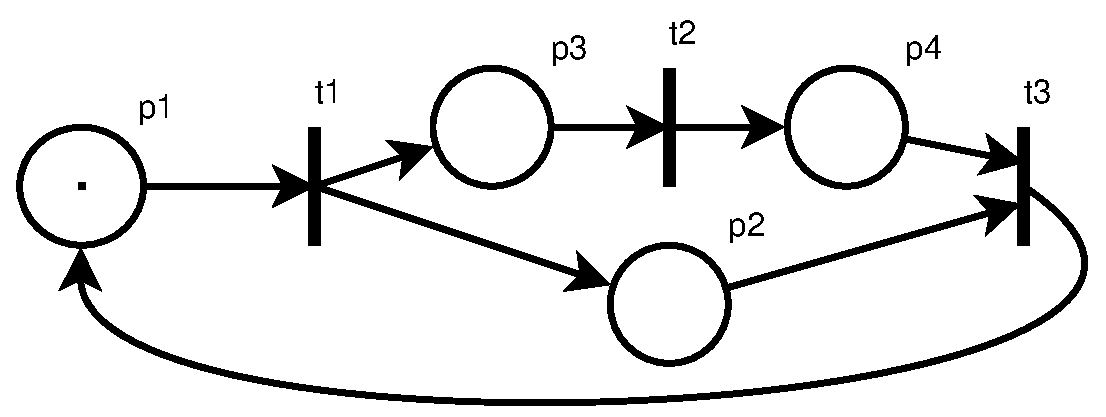
\includegraphics[width=0.5\textwidth]{Figures/OcultacionVsReduccion_1.eps}
\]
we can notice that $p_2$ is an implicit place because its marking can be
calculated as a function of $p_3$ y $p_4$:
\[
M(p_2) = M(p_3) + M(p_4)
\]
Moreover, by this same formula, it is clear that $ M (p_2) \geq M (P_4) $ (marking cannot be negative) so the only place that can prevent enabling of $ T_3 $ is $ P_4 $. Thus eliminating $ p_2$ does not alter the behavior of the network, which would be as follows:
\[
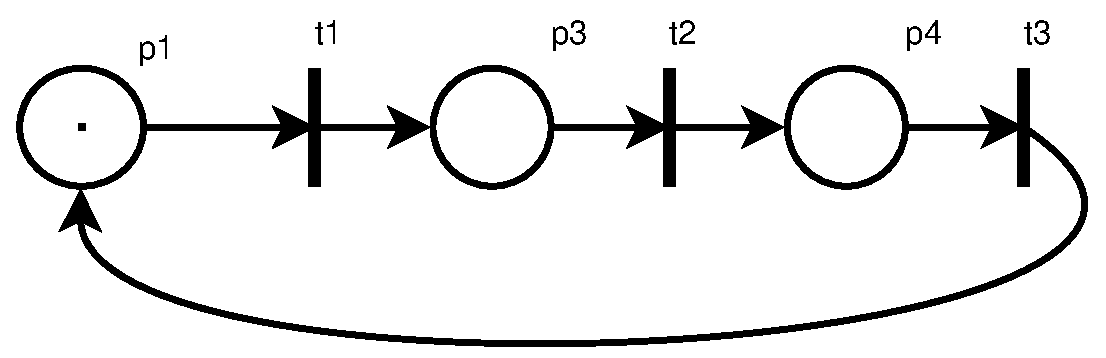
\includegraphics[width=0.5\textwidth]{Figures/OcultacionVsReduccion_2.eps}
\]
In this network elements have been removed, no hidden. This example helps us to see the difference between hiding and a reduction.
\end{example}  

\section{Conclusions}
As we have seen, any Petri net can be divided into any number of subnets, only limited by the number of places and transitions. Furthermore, each one of this Petri subnets has its own input and output front-ends in order to
connect with the rest of the Petri net.
Of course, the main application of this definitions in this thesis
is that the private information of this Petri net is stored in one or more
of these defined subnets.

 So I have reached the first milestone: to extend Petri Nets definition in order to define the public and the private information.  
